\documentclass[12pt]{article}
\usepackage{graphicx}
\usepackage{amsmath}
\usepackage{multicol}
\usepackage[right=1in,left=1in,top=1in,bottom=1in]{geometry}
\DeclareGraphicsExtensions{.pdf,.png,.jpg,.eps}
\begin{document}

\begin{center}
\textbf{Fourier Transforms} \\ 
Mitchell Miller \\
Illinois Institute of Technology \\
May 3 2012 {\ \\ \ \\}
\textbf{Abstract}\\
\end{center}
\noindent
Fourier analysis is an incredibly useful tool for studying periodic and many non-periodic systems.  This lab explores how the fast-fourier transform can be applied using to computer code to simulations and other problems.  First, the Van der Pol oscillator and damped, driven pendulum from the previous lab will be explored.  Then, the pseudo-spectral method will be used to simulate the effects of wave packet interactions with various potential wells.  Finally, a simulation exploring radar and sonar signal reflection and ranging will be presented.

\pagebreak

\section{Introduction}
\subsection{Discrete and Fast Fourier Transform}
The Fourier transform is used to express a function in terms of a new, independent variable. 
\begin{equation}
\label{four}
F[f(t)]=g(\omega)=\frac{1}{\sqrt{2\pi}} \int_{-\infty}^\infty f(t) e^{-i\omega t} dt
\end{equation}
It is common for Fourier transforms to be performed from time to frequency, as shown above.  One should note that a reverse Fourier transform is the same as \eqref{four} with $f(t)$ replaced with $g(\omega)$.  To convert \eqref{four} into a form applicable to computer work, one needs to convert the integral over all time into a sum
\begin{equation}
\label{fourSum}
f(t)=\sum_{-\infty}^\infty c_n e^{i n \pi t /T}
\end{equation}
where
\begin{equation}
\label{fourCoef}
c_n = \frac{1}{2T} \int_{-T}^T f(t) e^{-i n \pi t /T}
\end{equation}
From this, we can find that the discrete frequency steps are defined as
\begin{equation}
\label{Omeg}
\omega = \frac{n\pi}{T}
\end{equation}
To apply this to a real application over a domain $0<t<T$ with $N$ discrete points, one can approximate \eqref{fourSum} with the trapezoid rule to define a Discrete Fourier Transform (DFT)
\begin{equation}
\label{fourDis}
g(n \Delta \omega) = \sum_{m=0}^{N-1} f(m \Delta t) e^{-2 \pi i m n/N}
\end{equation}
where $\Delta \omega = \frac{2 \pi}{T}$.  This limits the resolution so that only frequency less than or equal to $(N-1)\Delta \omega /2$.  In this limit, the factor of two originates from a phenomenon called the Nyquist frequency.  
\begin{equation}
\label{nyq}
\omega_{Nyquist} = \frac{N \Delta \omega}{2}
\end{equation}
Any frequency beyond $\omega_{Nyquist}$ are the negative frequencies from $-N \Delta \omega/2$ to $-\Delta \omega$.  When observing a plot of a transformed function, this phenomenon manifests as a reflection about $\omega_{Nyquist}$.

Although this is a viable method for performing Fourier transforms, the number of operations required goes as $N^2$, making large computation times prohibitively large for large data sets.  Fortunately, there is another method to calculate Fourier transforms called the Fast-Fourier Transform (FFT).  To begin, the sum used to calculate a DFT is split into two sums, one over even and one over odd indices:  $m=2j$ for the even sum and $m=2j+1$ for the odd.  It turns out that each of these new sums are also DFT, but now the number of operations is only $(N/2)^2$ for each, reducing the total number of operations by a half.  However, this splitting between even and odd indices can be repeated as long as each sum has an even number of terms.  So, for an FFT with $N=2^k$ points, the number of operations required is not $N^2$, but $N$log$_2 N$.
\subsection{Pseudo Spectral Method}
The pseudo spectral method is a technique to analyze a problem using FFT's.  For this lab, several quantum mechanical scattering problems will be explored.  First, one defines the Schronidger equation in terms of the kinetic and potential energy operators $\mathbf{T}$ and $\mathbf{V}$, respectively.
\begin{equation}
\label{Schro}
i \hbar \frac{\partial \psi(x,t)}{\partial t} = (\mathbf{T} + \mathbf{V})\psi(x,t)
\end{equation}
This problem was solved in the previous lab using alternate methods, but the pseudo spectral method presents a new and potentially more efficient method for solving it.  It is known that the exact solution to \eqref{Schro} is 
\begin{equation}
\label{SchroSoln}
\psi(x,t)=e^(-i(\mathbf{T}+\mathbf{V})\delta_t/\hbar)
\end{equation}
where $\delta_t$ is a time step used for calculating the time evolution of the wave function.  Unfortunately, since $\mathbf{T}$ and $\mathbf{V}$ are operators, this cannot be separated into the product of two exponential functions.  To generate the form to this solution via the pseudo spectral method, first an approximation to $\psi(x,t)$ must be defined
\begin{equation}
\label{psiApprox}
\psi(x,t)\approx e^{-i\mathbf{V}\delta_t/2\hbar}e^{-i\mathbf{T}\delta_t/\hbar}e^{-i\mathbf{V}\delta_t/2\hbar} \psi(x,t_0)
\end{equation}
For $j$ points being evaluated in an FFT, an intermediate function can be defined
\begin{equation}
\label{phi}
\phi(x_j)=e^{-i V(x_j)\delta_t/2\hbar} \psi(x_j,t_0)
\end{equation}
From here, $\phi$ must be multiplied by the next term in \eqref{psiApprox}, which contains the kinetic operator.  In coordinate space, this is avery difficult term to evaluate since there is a differential in an exponent.  However, if one transforms this expression, it becomes fairly trivial.  
\begin{equation}
\label{kineticPhi}
e^{-i\mathbf{T}\delta_t/\hbar} \phi(x) = F^{-1}[e^{-i T(k) \delta_t /\hbar} \Phi(k)]
\end{equation}
where $T(k)=\frac{\hbar^2 k^2}{2m}$ and 
\begin{equation}
\label{PHI}
\Phi(k) = F[\phi(x)]
\end{equation}
Finally, this is multiplied by the third exponential term in the approximation, to find
\begin{equation}
\label{fullPsi}
\psi(x,t) \approx e^{-i V(x) \delta_t/2\hbar} F^-1[e^{-i T(k)\delta_t/\hbar} F[e^{-i V(x) \delta_t /2\hbar} \psi(x,t_0)]]
\end{equation}
From this, one can set a $V(x)$ and calculate the solution with relative ease.
\subsection{Cross Correlation}
Correlation is a measure of how similar two functions or data sets are.  This is a very useful tool for studying signals in noise, and will be applied to a ranging problem later in this lab.  The correlation between two functions, $f(t)$ and $g(t)$, is defined as
\begin{equation}
\label{correl}
f(t) \odot g(t) = \frac{1}{\sqrt{2\pi}} \int_{-\infty}^\infty f^*(\tau)g(t+\tau)d\tau
\end{equation}
To convert this integral into something usable in computer code, the trapezoid rule is applied, leaving just a few lines of simple code.

\section{Applications}
\subsection{Van der Pol Oscillator}
The first application of FFTs is the analysis of the Van der Pol Oscillator.  This system was presented in the last lab as a demonstration of chaotic motion.  Using code developed earlier, a list of position versus time values was generated for use to demonstrate applications in FFT.
\begin{figure}[!h]
\centering
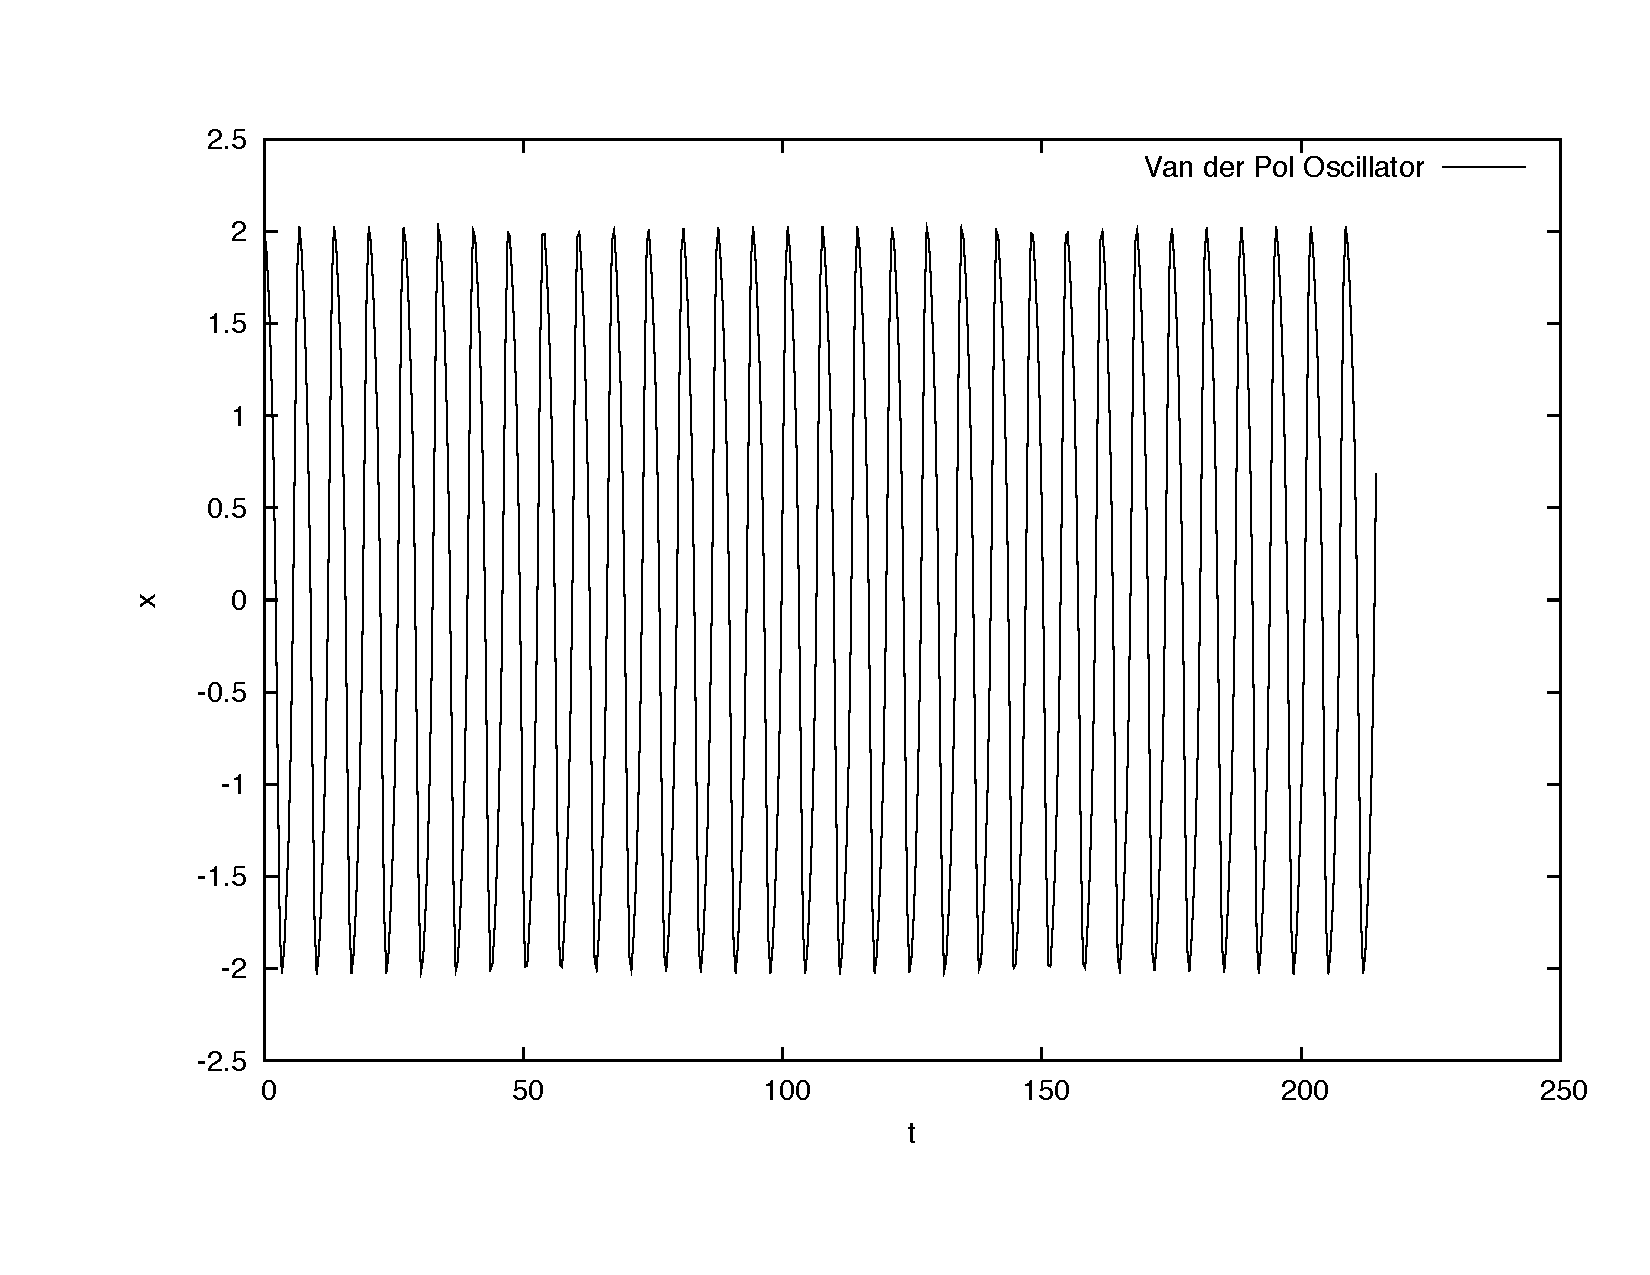
\includegraphics[width =120 mm, height = 75mm]{van.pdf}
\caption{Position versus time plot for the Van der Pol Oscillator.}
\label{fig:van}
\end{figure}
\begin{figure}[!h]
\centering
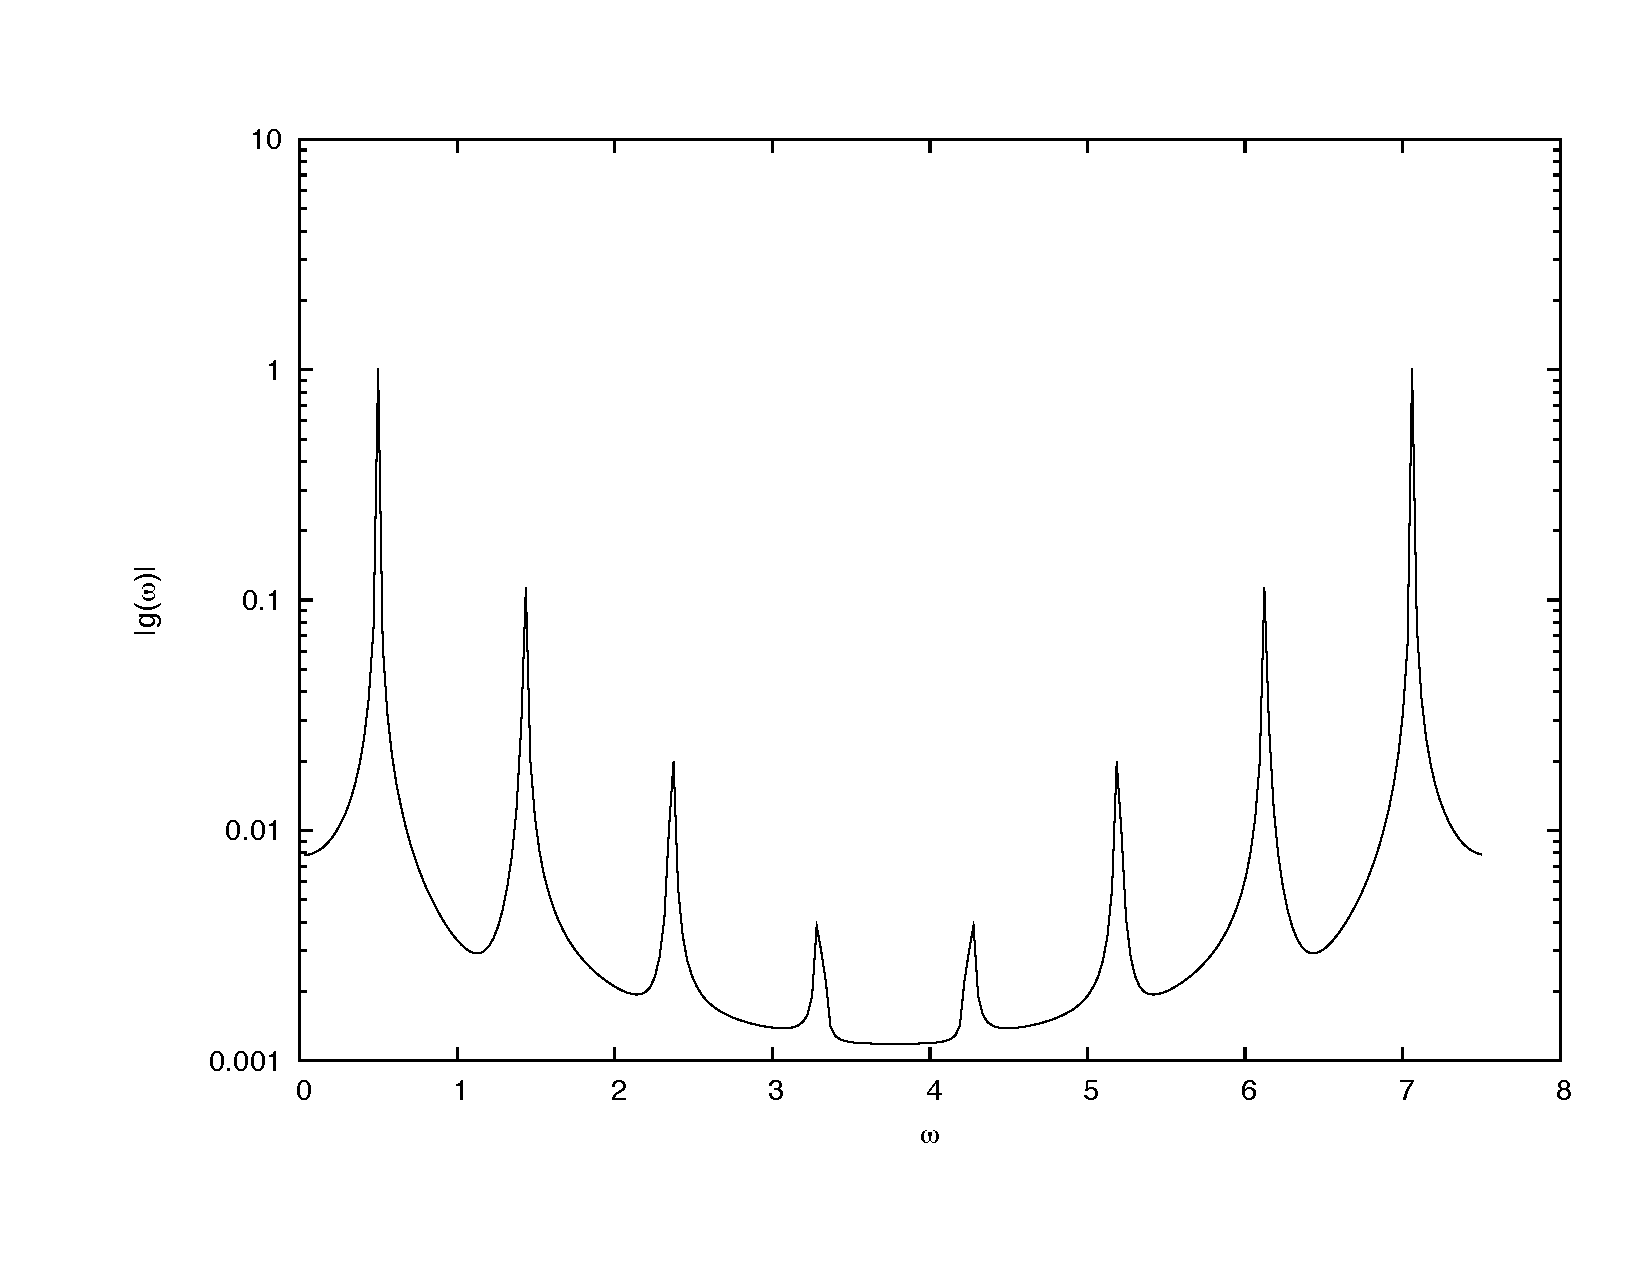
\includegraphics[width =120 mm, height = 75mm]{Fig_6_18.pdf}
\caption{Frequency spectrum of \ref{fig:van} using a sampling period in sync with oscillator.}
\label{fig:618}
\end{figure}

Using the data contained in Fig. \ref{fig:van}, a frequency spectrum was obtained via the FFT method.  These results are shown in Fig. \ref{fig:618}.  If the input were a perfect sinusoidal function, there would be a single peak in the frequency spectrum.  However, the shape of the Van der Pol Oscillator is not, so the frequency spectrum shows several peaks at different values.  If Fig. \ref{fig:618} is examined closely, one will notice a clear point at which the spectrum reflects around the Nyquist frequency.  For the sampling parameters used in this FFT, $\omega_{Nyquist} = 3.75$, which matches what one observes in the spectrum.
\subsection{Damped Driven Pendulum}
The next application of basic FFT is the damped, driven pendulum, another system that was explored in the previous lab.  This system is one of the classic demonstrations of chaotic behavior.  An FFT was performed for several different values of $F_D$, showing frequency space as the system becomes chaotic.  
\begin{figure}[!h]
\centering
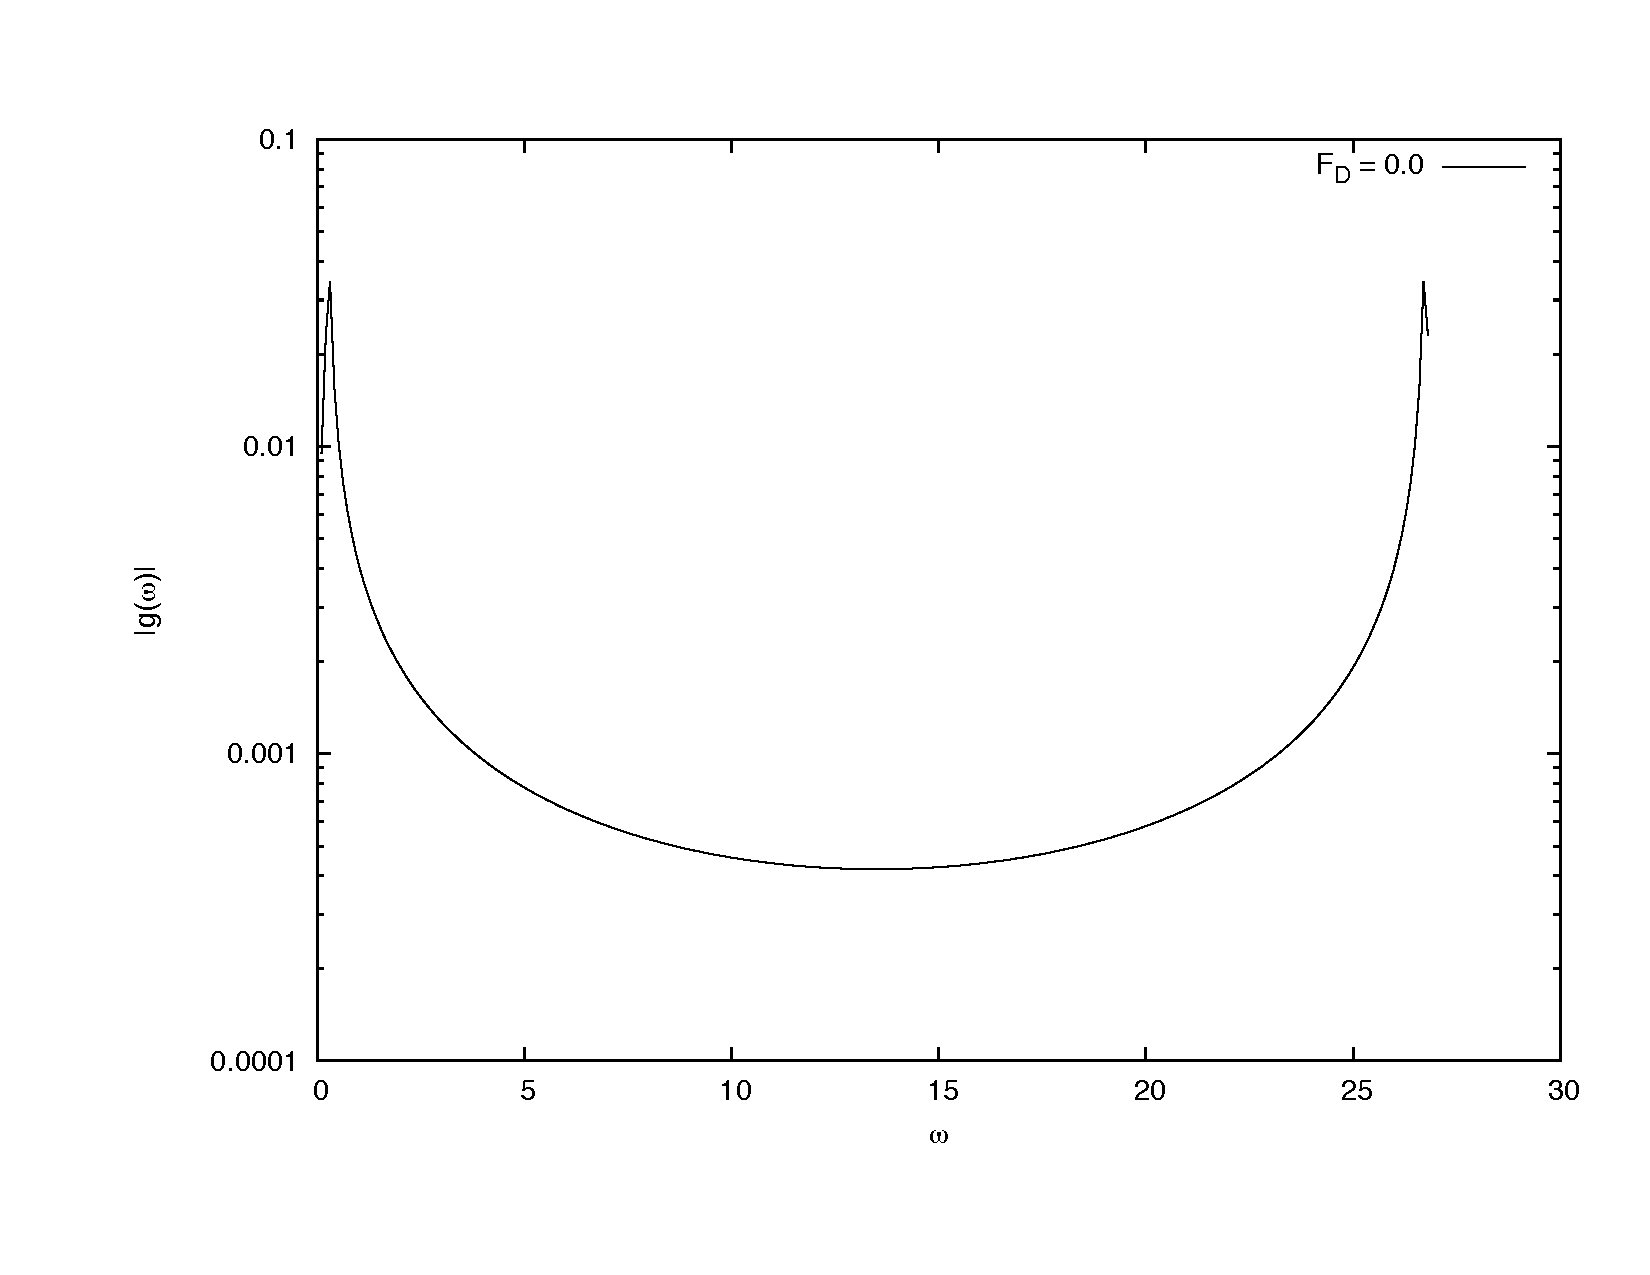
\includegraphics[width =120 mm, height = 75mm]{ddp_0.pdf}
\caption{Frequency spectrum for the damped driven pendulum with $F_D = 0.0$.}
\label{fig:0}
\end{figure}
\begin{figure}[!h]
\centering
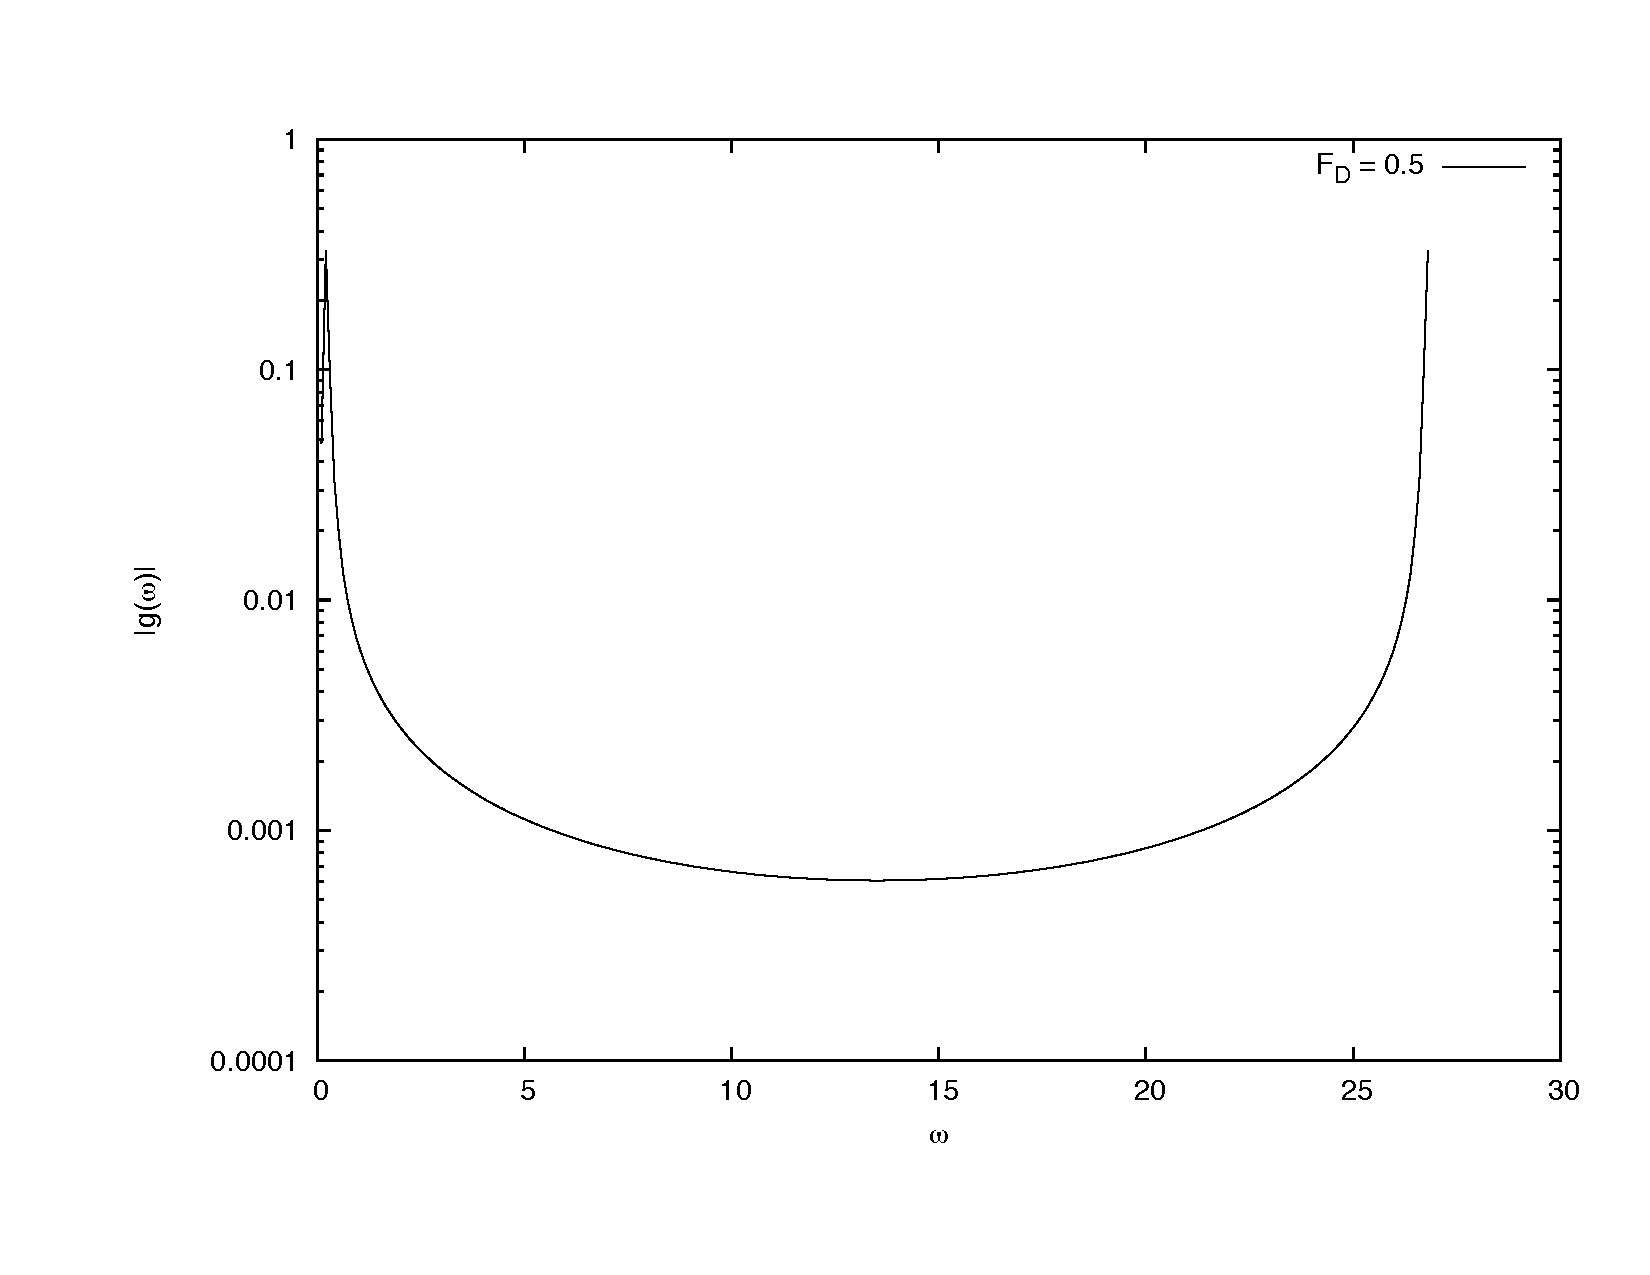
\includegraphics[width =120 mm, height = 75mm]{ddp_5.pdf}
\caption{Frequency spectrum for the damped driven pendulum with $F_D = 0.5$.}
\label{fig:5}
\end{figure}
\begin{figure}[!h]
\centering
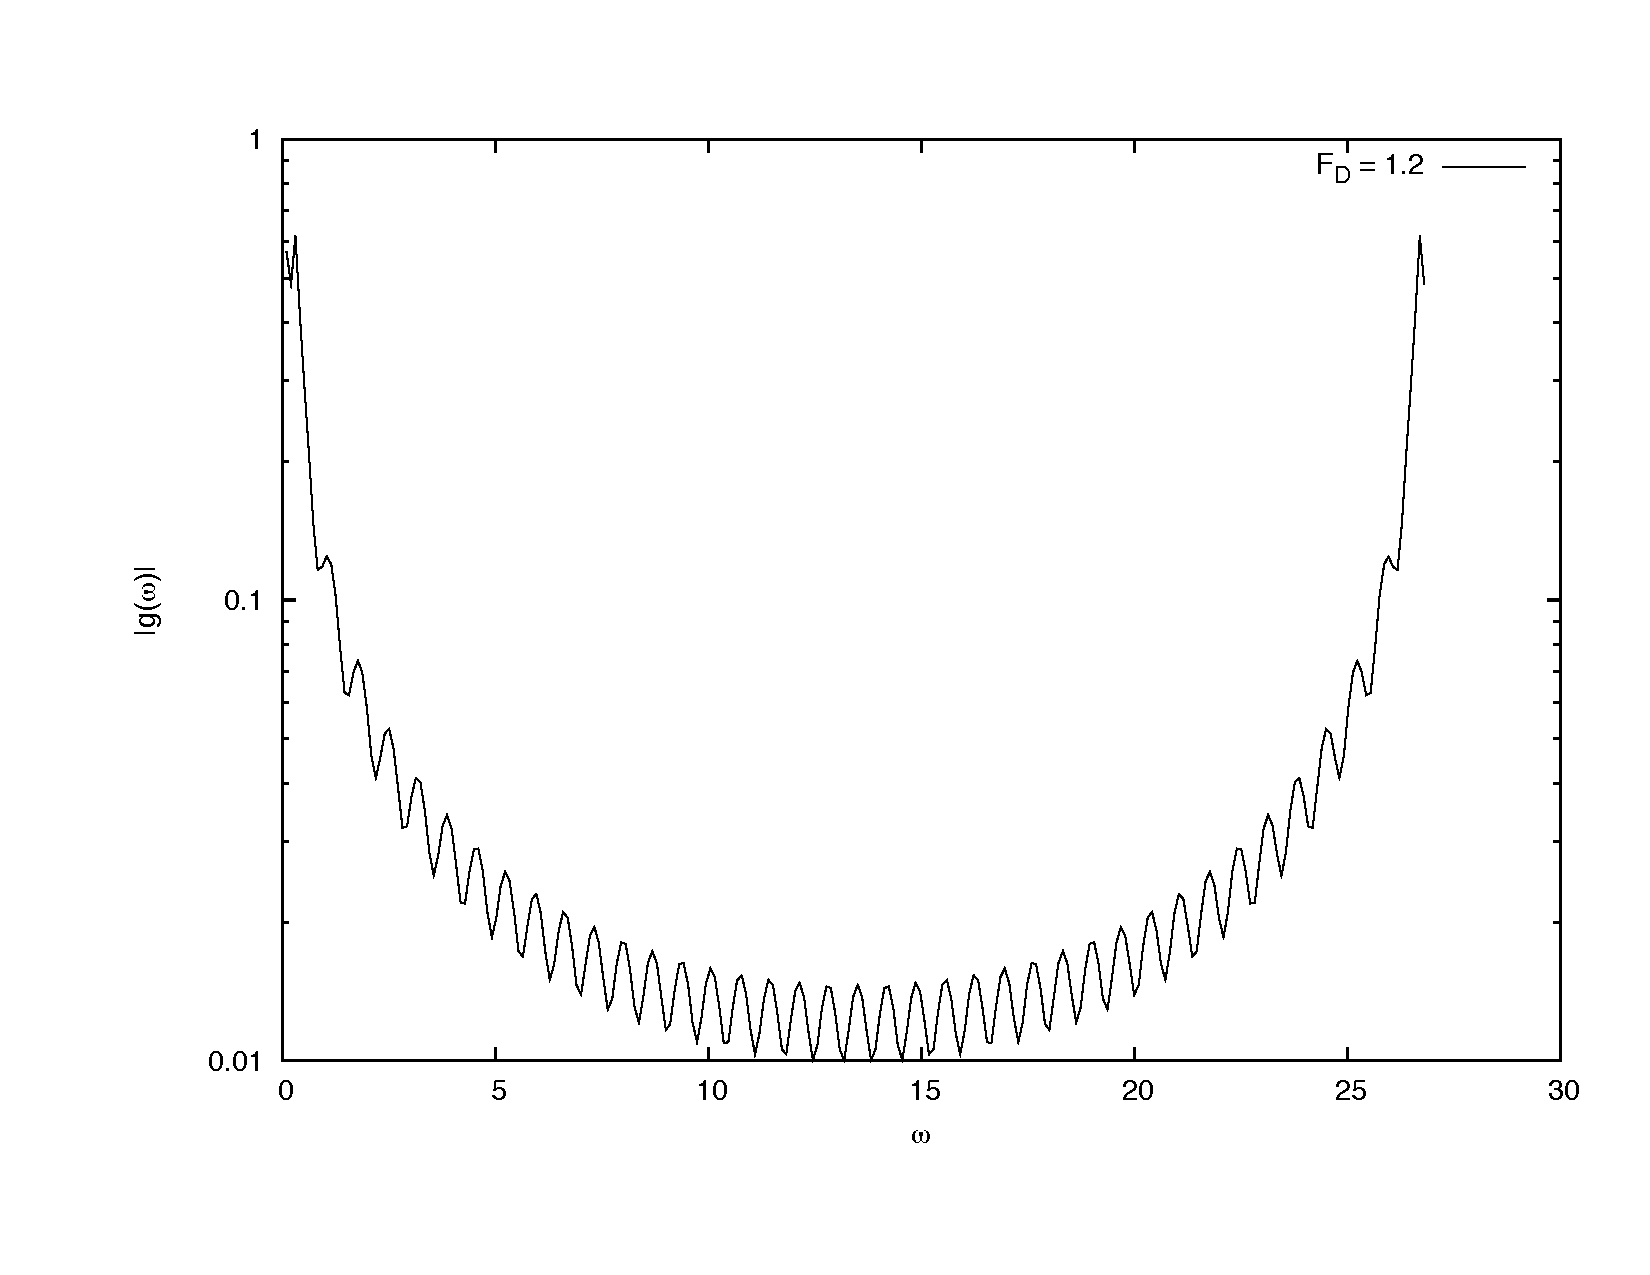
\includegraphics[width =120 mm, height = 75mm]{ddp_12.pdf}
\caption{Frequency spectrum for the damped driven pendulum with $F_D = 1.2$.}
\label{fig:12}
\end{figure}

Figures \ref{fig:0} through \ref{fig:12} show the frequency spectra for $F_D = 0.0$, $0.5$, and $1.2$.  From the previous lab, it was determined that this system does not become chaotic until relatively high values of $F_D$ ( $>$ 1).  If the previous lab is used as a reference, the system is 'most periodic' when $F_D = 0.5$.  When $F_D = 0.0$, the damping force quickly overwhelms the motion, and the oscillations quickly decay to nothing.  Finally, when $F_D = 1.2$, the motion has very little obvious periodic behavior, with wild oscillations in chaos.  

These results are reflected in the frequency spectra as well.  Fig. \ref{fig:5} shows the most clean spectra, with well defined peaks, corresponding to a highly periodic function.  Fig. \ref{fig:0} shows a bit more broad peak shapes, which match the oscillators behavior of a decaying motion.  FInally, Fig. \ref{fig:12} shows many, many peaks at varying frequencies, which meet the expect results of a chaotic system.
\subsection{Quantum Barriers}
The pseudo spectral technique described earlier was applied to several quantum mechanical barrier problems.  The first was scattering of a wave packet with energy less than the magnitude of the well.  This problem demonstrates evanescent wave behavior, meaning that, at the point of collision, some part of the wave packet actually exists in the barrier, where it would be forbidden classically.
\begin{figure}[!h]
\centering
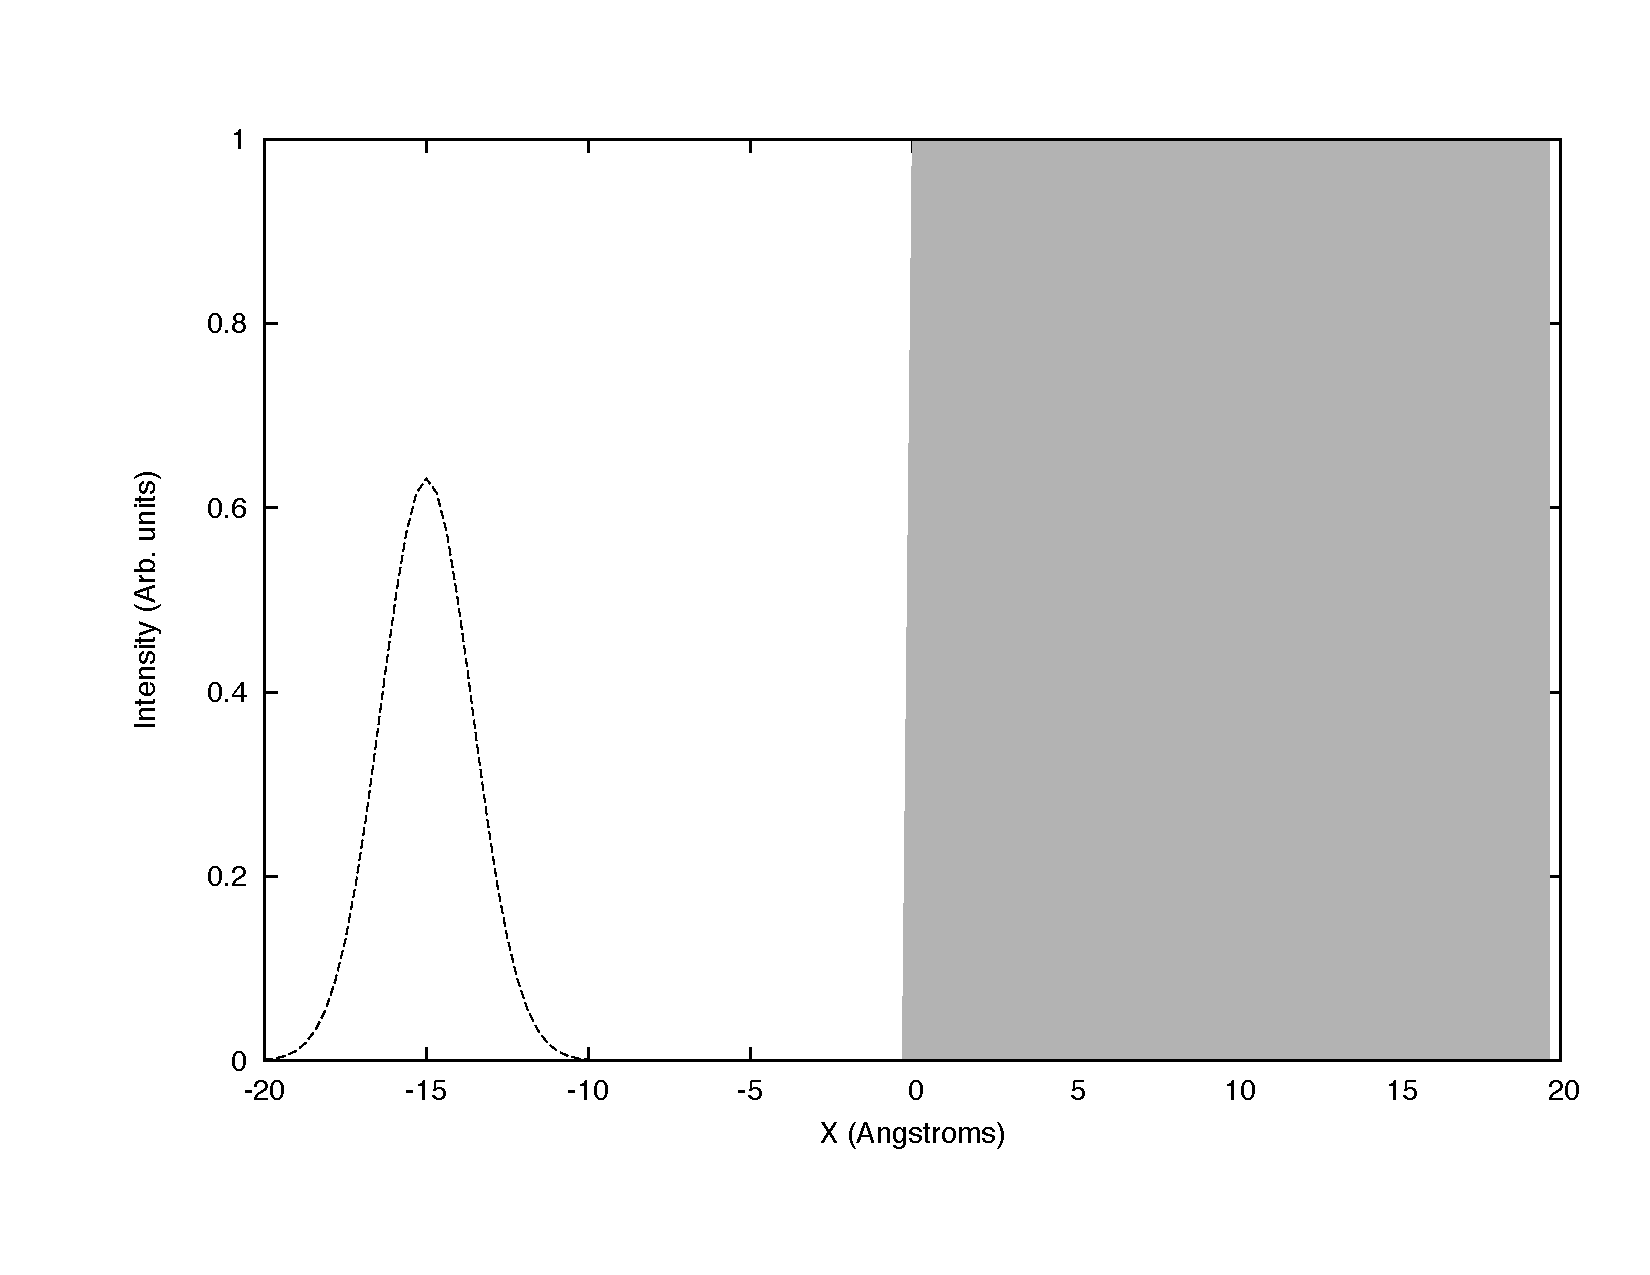
\includegraphics[width =120 mm, height = 75mm]{Ex_7_21_start.pdf}
\caption{Initial state of a wave packet with energy less than the potential barrier.}
\label{fig:721s}
\end{figure}
\begin{figure}[!h]
\centering
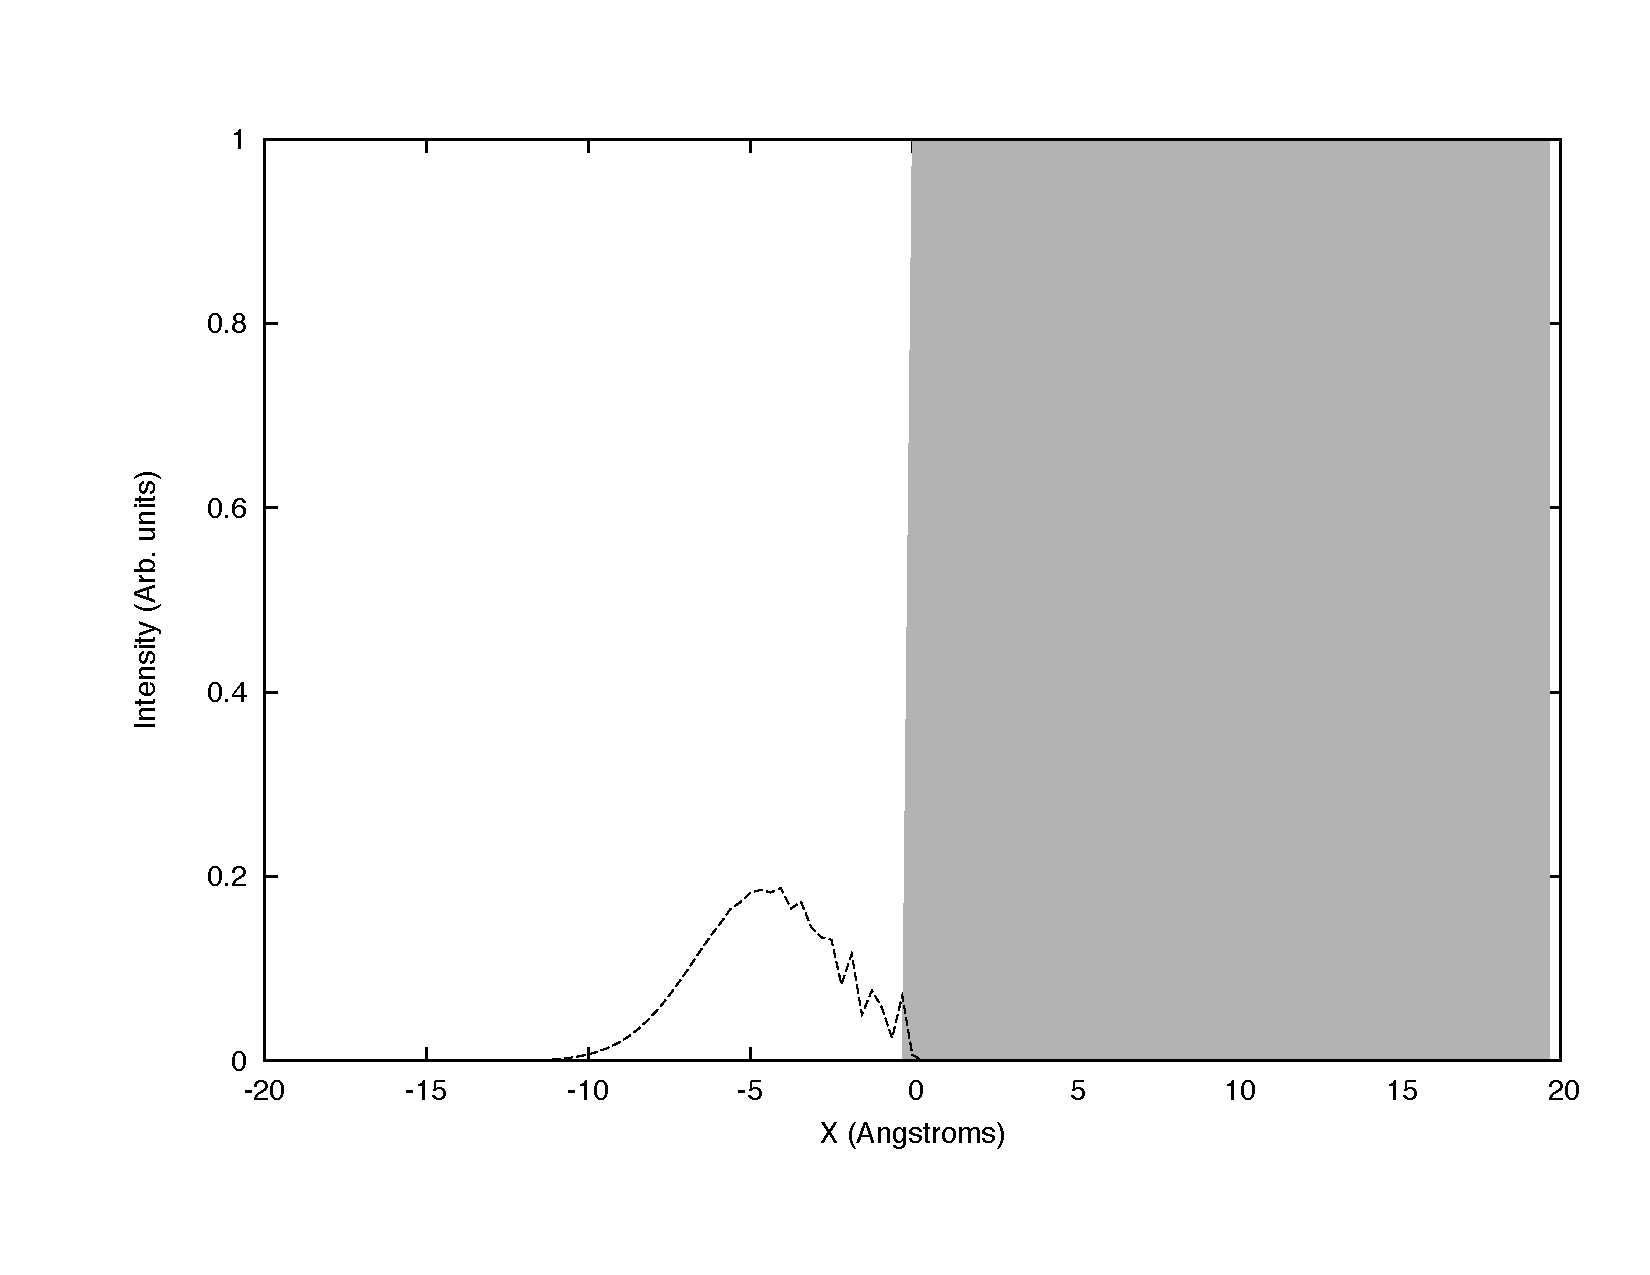
\includegraphics[width =120 mm, height = 75mm]{Ex_7_21_end.pdf}
\caption{Interference between a wave packet with energy less than the potential barrier and the barrier.}
\label{fig:721e}
\end{figure}

Fig. \ref{fig:721e} shows the behavior of the packet upon contact with the barrier.  Note that there a nonzero intensity inside the barrier at $x>0$.  As more time passes in this simulation, the wave is then reflected back towards its starting position, shown in Fig. \ref{fig:721s}.

\begin{figure}[!h]
\centering
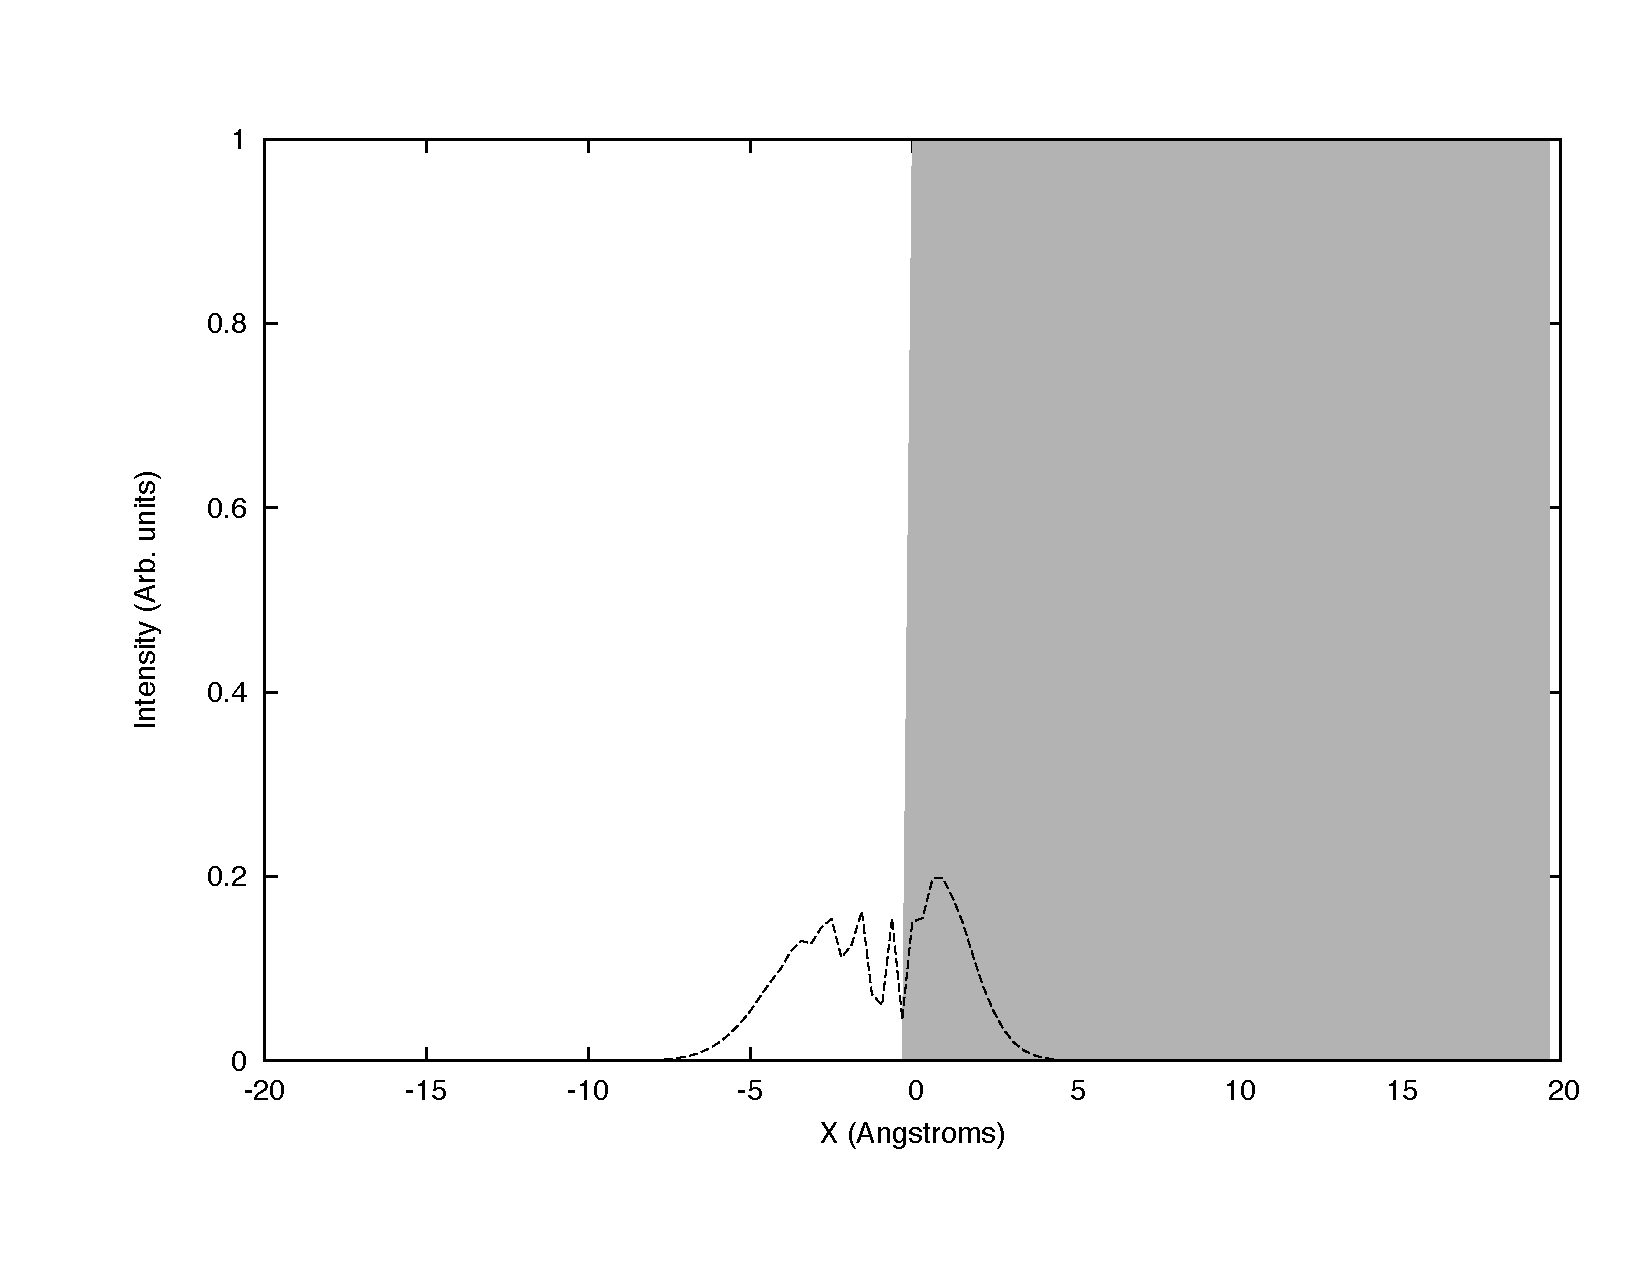
\includegraphics[width =120 mm, height = 75mm]{Ex_7_23_collis.pdf}
\caption{Interference between a wave packet with energy greater than a barrier and the potential barrier.}
\label{fig:723c}
\end{figure}
\begin{figure}[!h]
\centering
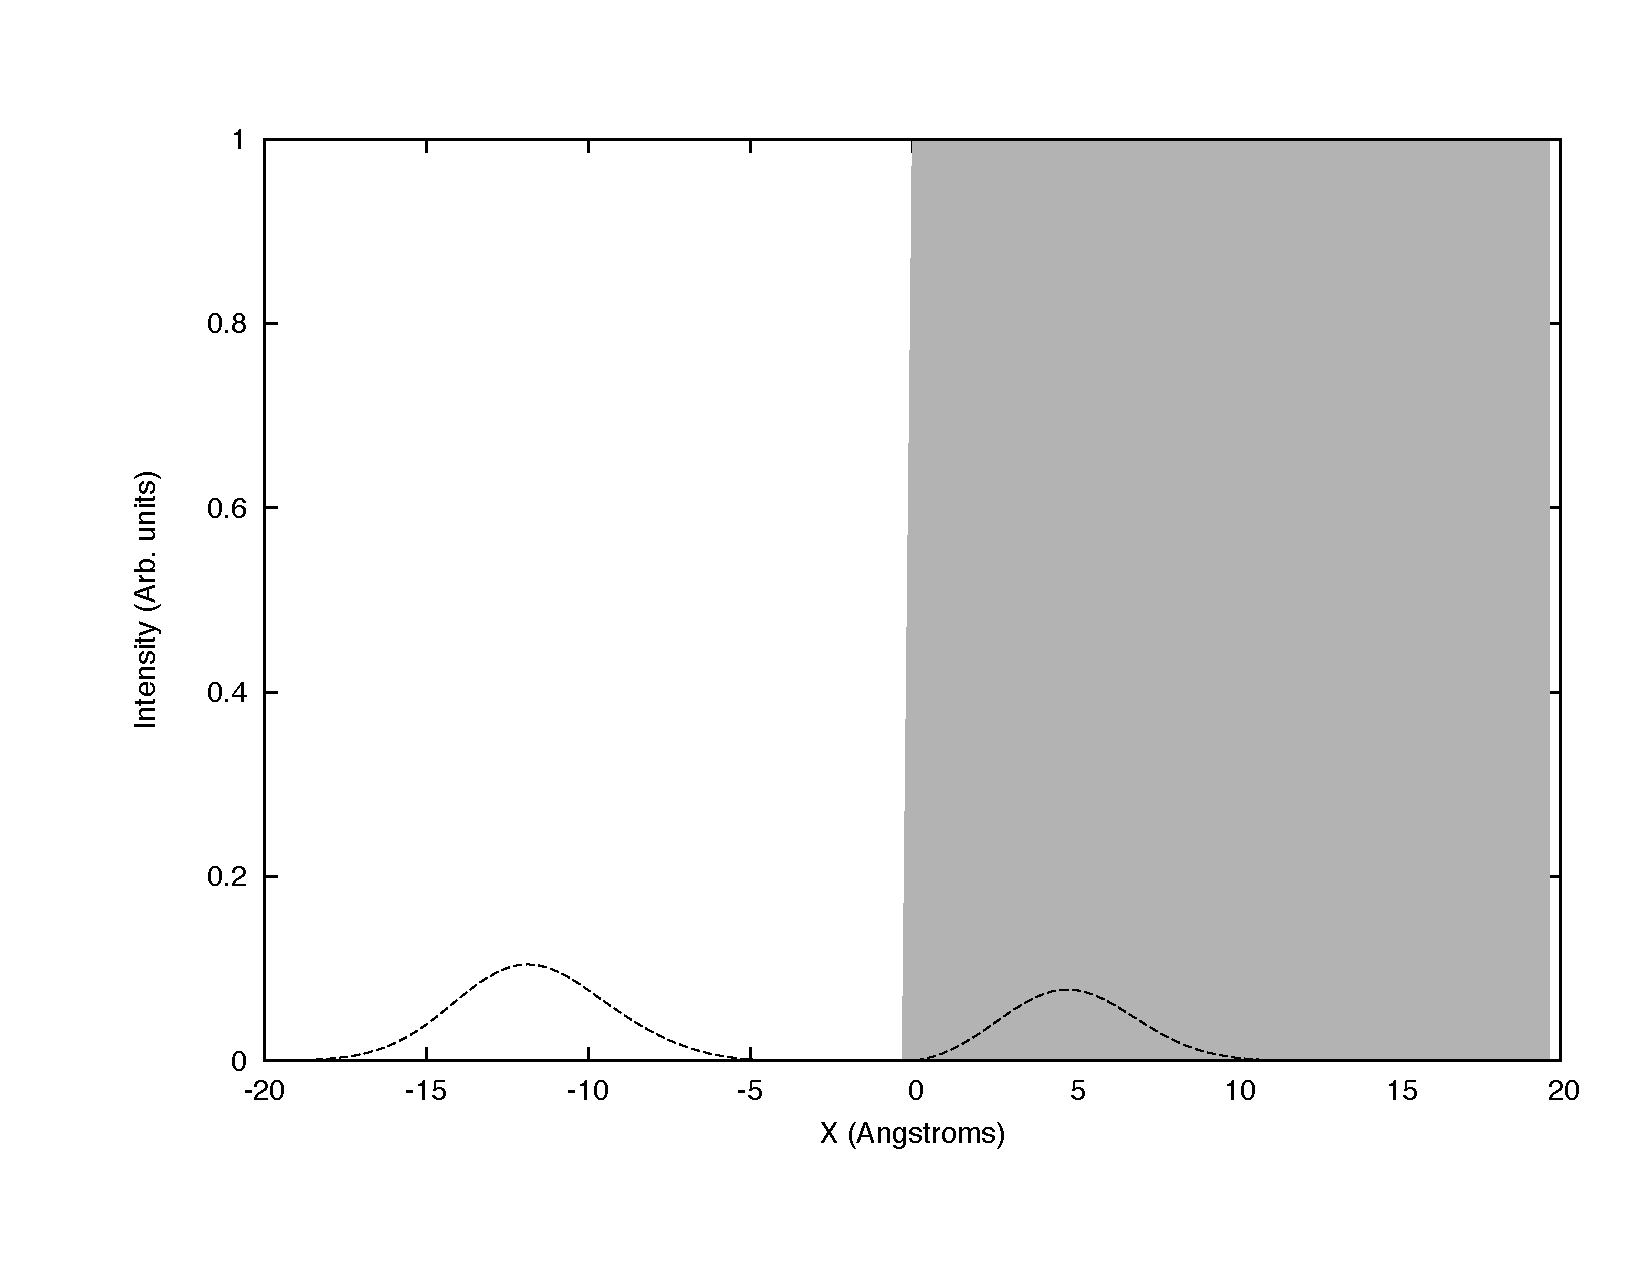
\includegraphics[width =120 mm, height = 75mm]{Ex_7_23_reflec.pdf}
\caption{Reflection and transmission of the wave packet after meeting the potential barrier.}
\label{fig:723r}
\end{figure}

Figures \ref{fig:723c} and \ref{fig:723r} show how the wave packet interacts with a barrier when the packet's energy is greater than the size of the barrier.  At the moment when the packet reaches the barrier, Fig. \ref{fig:723c} shows the interference effects between the packet and the barrier.  After the wave has passed over the barrier, it separates into a reflected (peak to the left of the barrier traveling left) and a transmitted (peak to the right of barrier traveling right) packet.  This is shown in Fig. \ref{fig:723r}.  Note that the transmitted packet has a smaller intensity, due to the effect of the barrier.

Next, a potential well was explored.  This system has similar properties to the wave packet meeting a potential well when the packet's energy is greater than the well.  Again, one sees interference with the well and the wave packet when they first meet, shown in Fig. \ref{fig:726c}.  This interference becomes a reflection and transmission as the wave passes over the well, shown in Fig. \ref{fig:726r}.

\begin{figure}[!h]
\centering
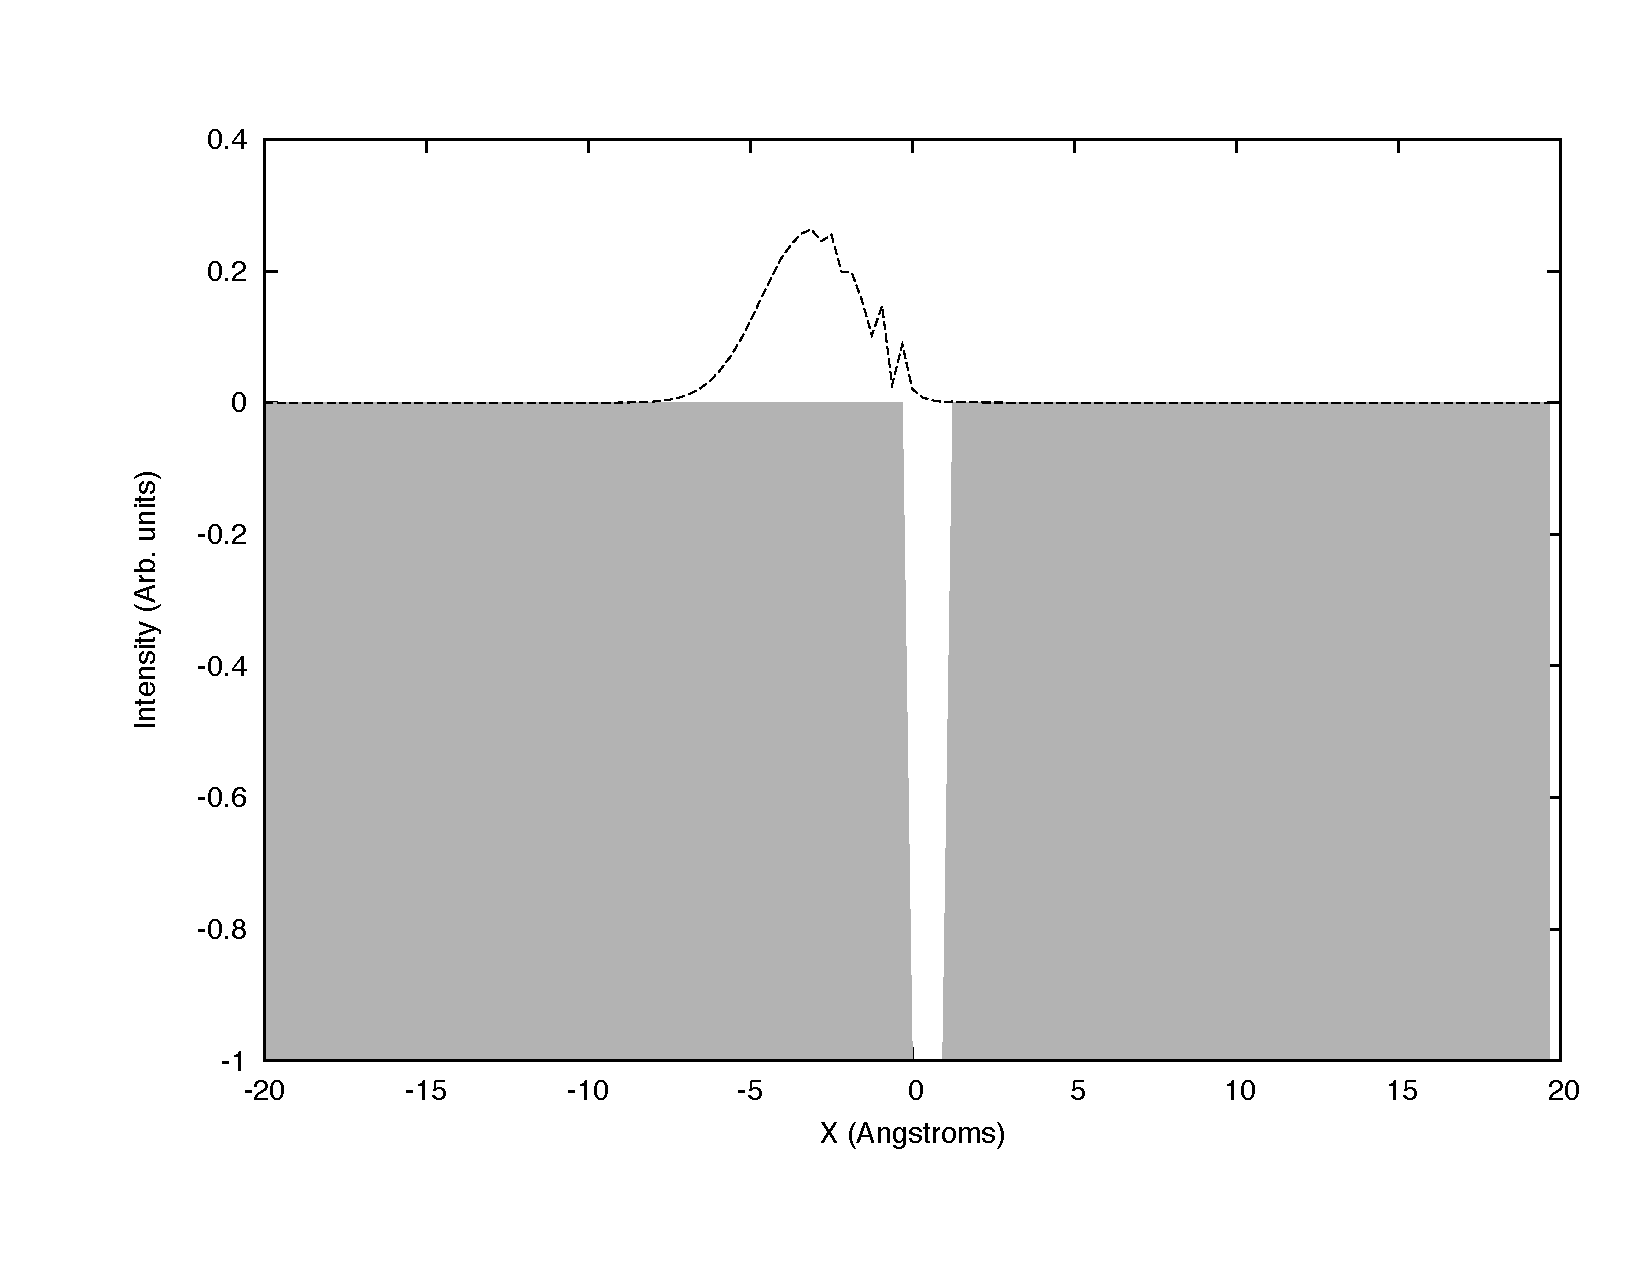
\includegraphics[width =120 mm, height = 95mm]{Ex_7_26_collis.pdf}
\caption{Wave packet meeting a potential well.}
\label{fig:726c}
\end{figure}
\begin{figure}[!h]
\centering
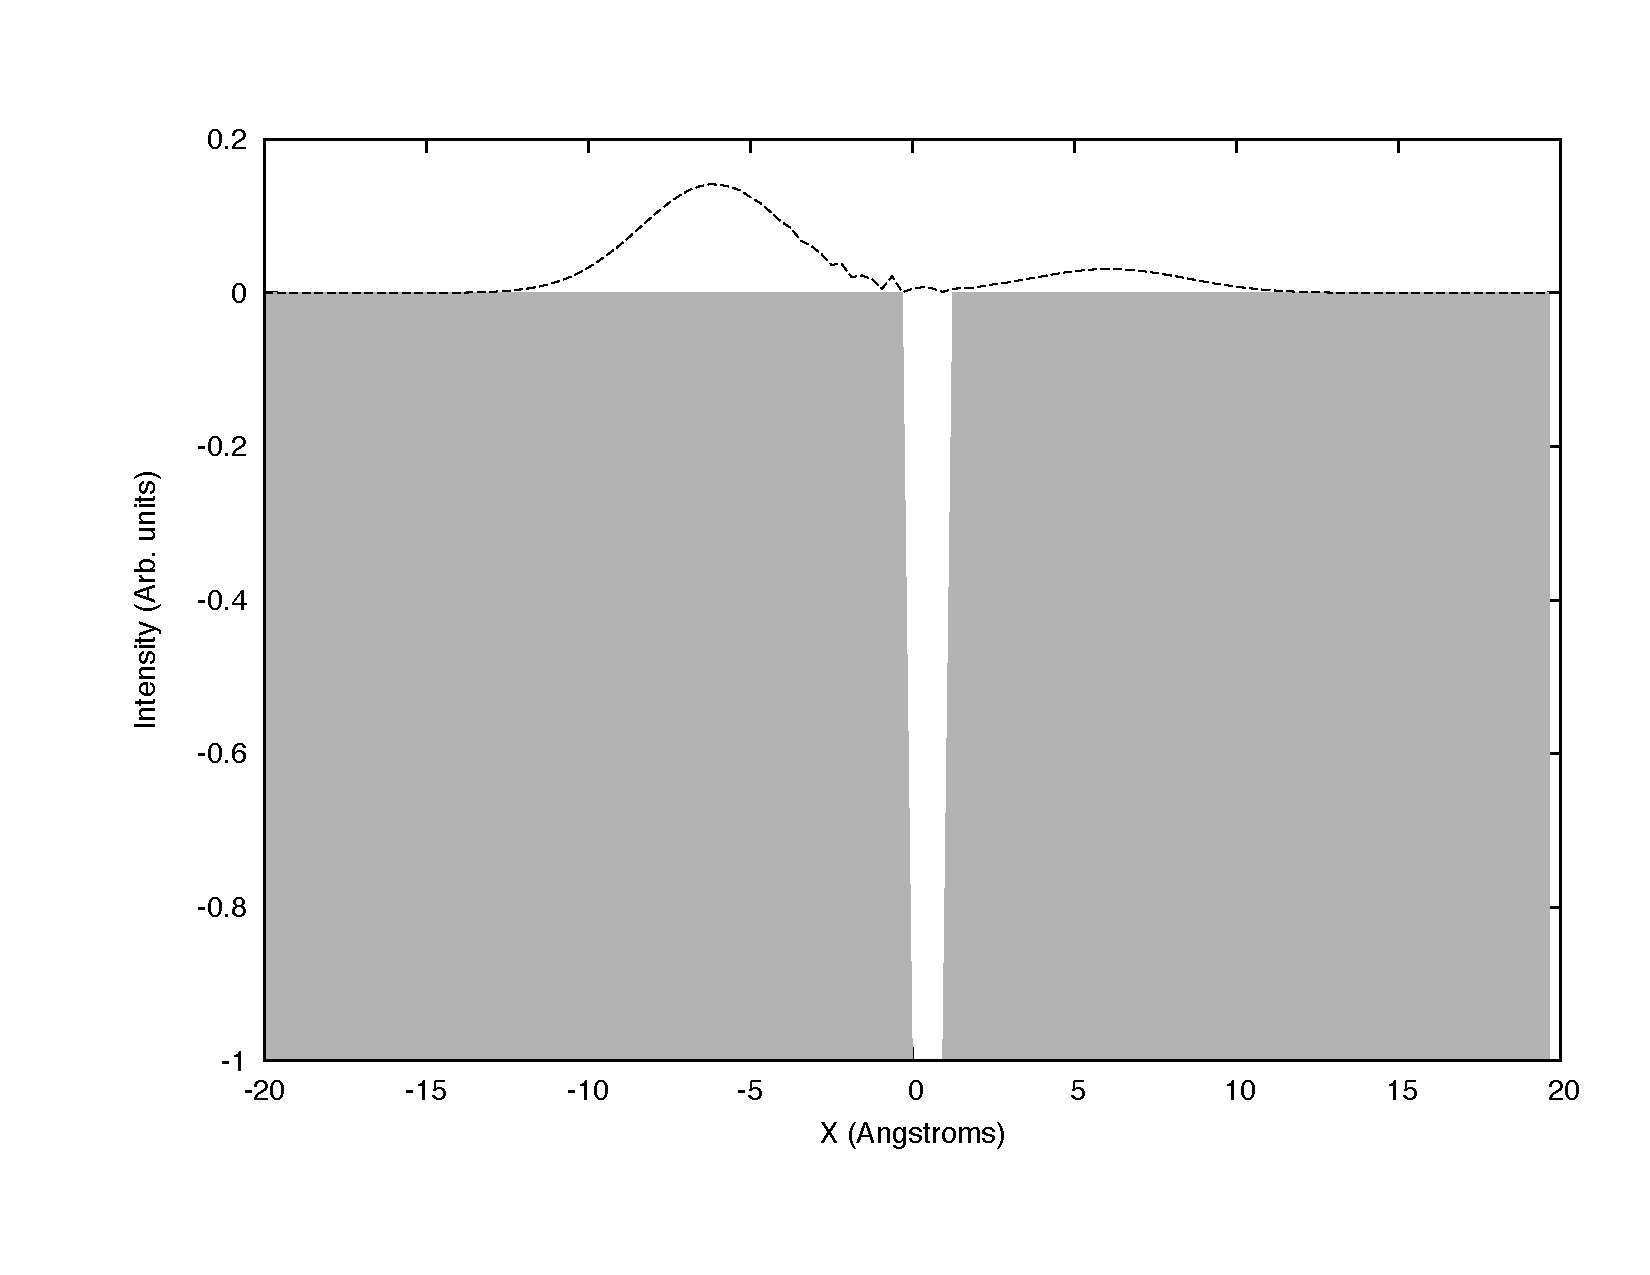
\includegraphics[width =120 mm, height = 95mm]{Ex_7_26_reflec.pdf}
\caption{Reflection and transmission of the wave packet after passing over the potential well.}
\label{fig:726r}
\end{figure}

The final situation explored with the pseudo spectral method was a narrow potential barrier.  Two wave packets, one with energy less than and one with energy greater than the barrier, were simulated.  When the packet's energy is less than the barrier's very little is transmitted through it.  This can be seen in Fig. \ref{fig:728r}.  A log scale is used because the transmission wave is orders of magnitude less than the reflected wave.  However, when the packet's energy is greater than the barrier's, there is a clear transmission component.  Unfortunately, an error in the code or an artifact of the method caused some wave to remain within the barrier, as can be seen in Fig. \ref{fig:729r}.


\begin{figure}[!h]
\centering
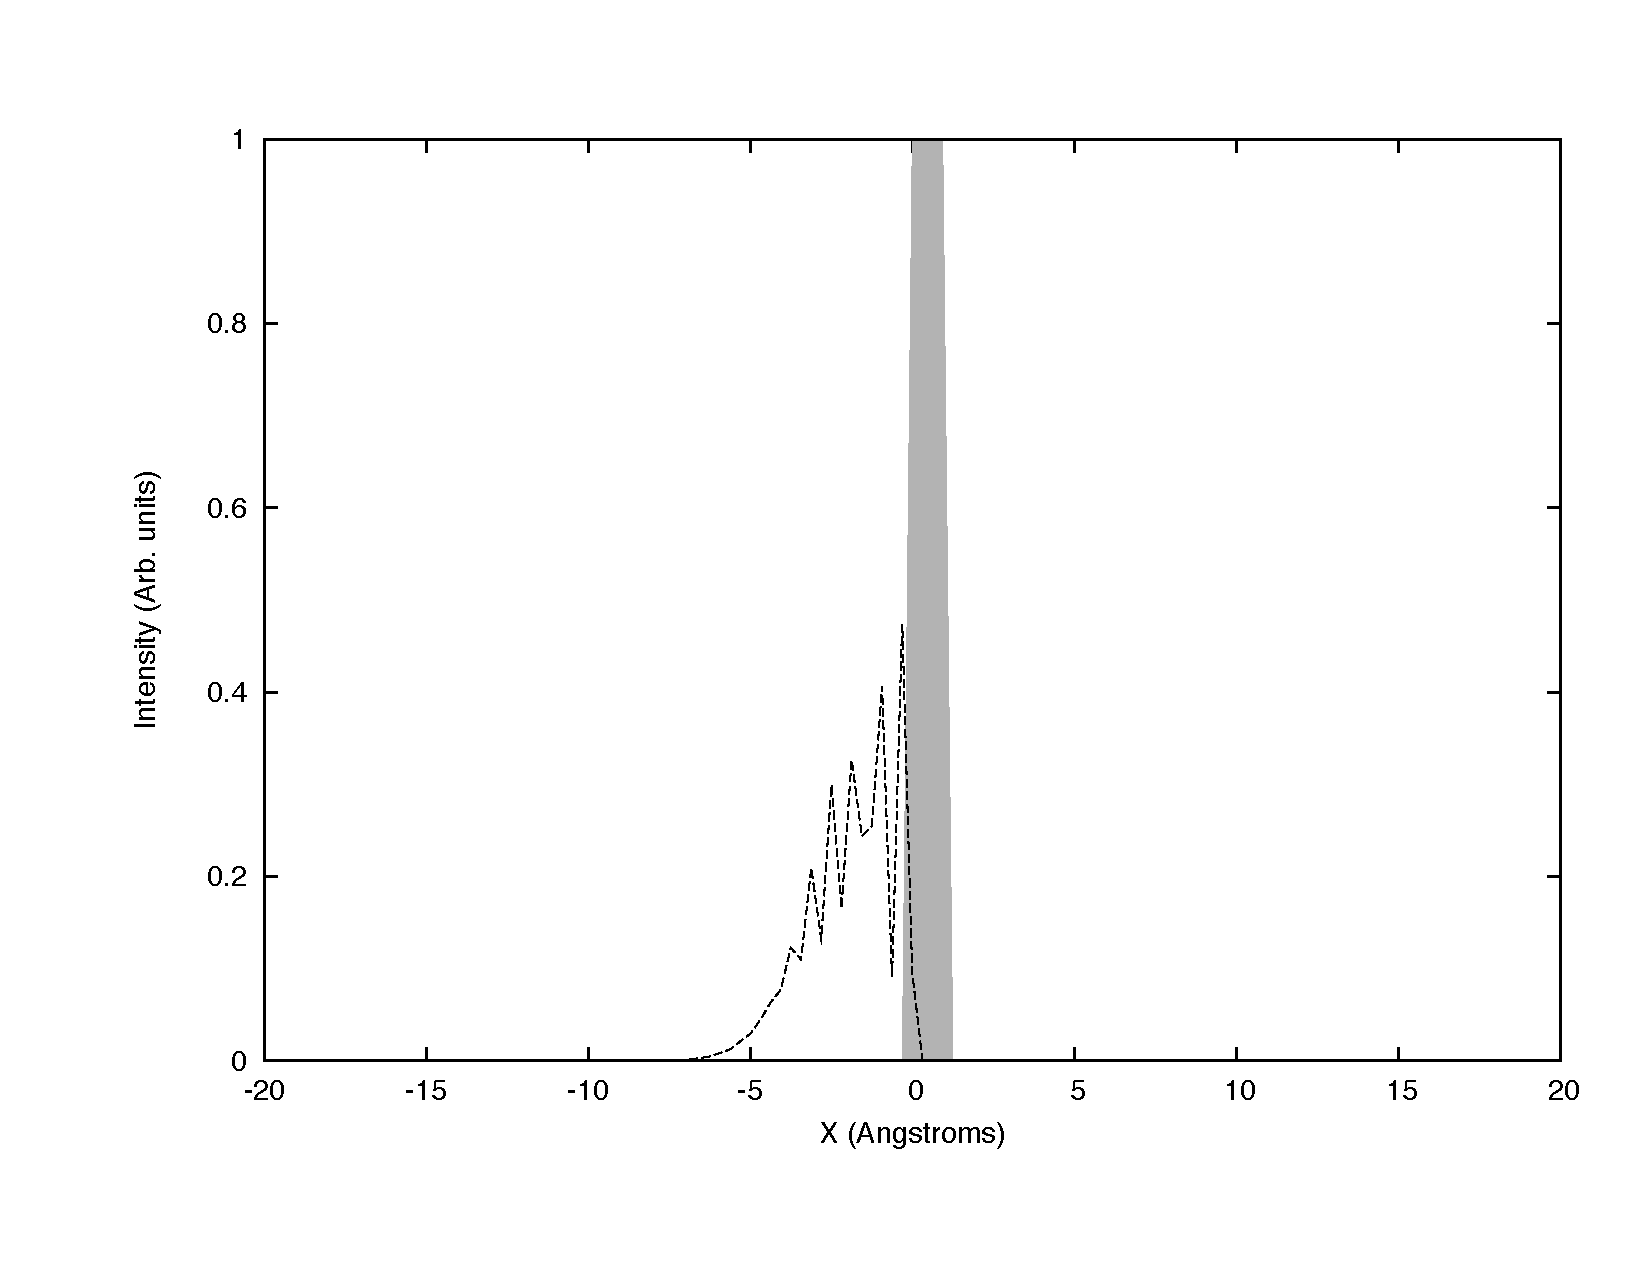
\includegraphics[width =120 mm, height = 95mm]{Ex_7_28_collis.pdf}
\caption{Wave packet meeting a thin potential barrier with energy less than the barrier.}
\label{fig:728c}
\end{figure}
\begin{figure}[!h]
\centering
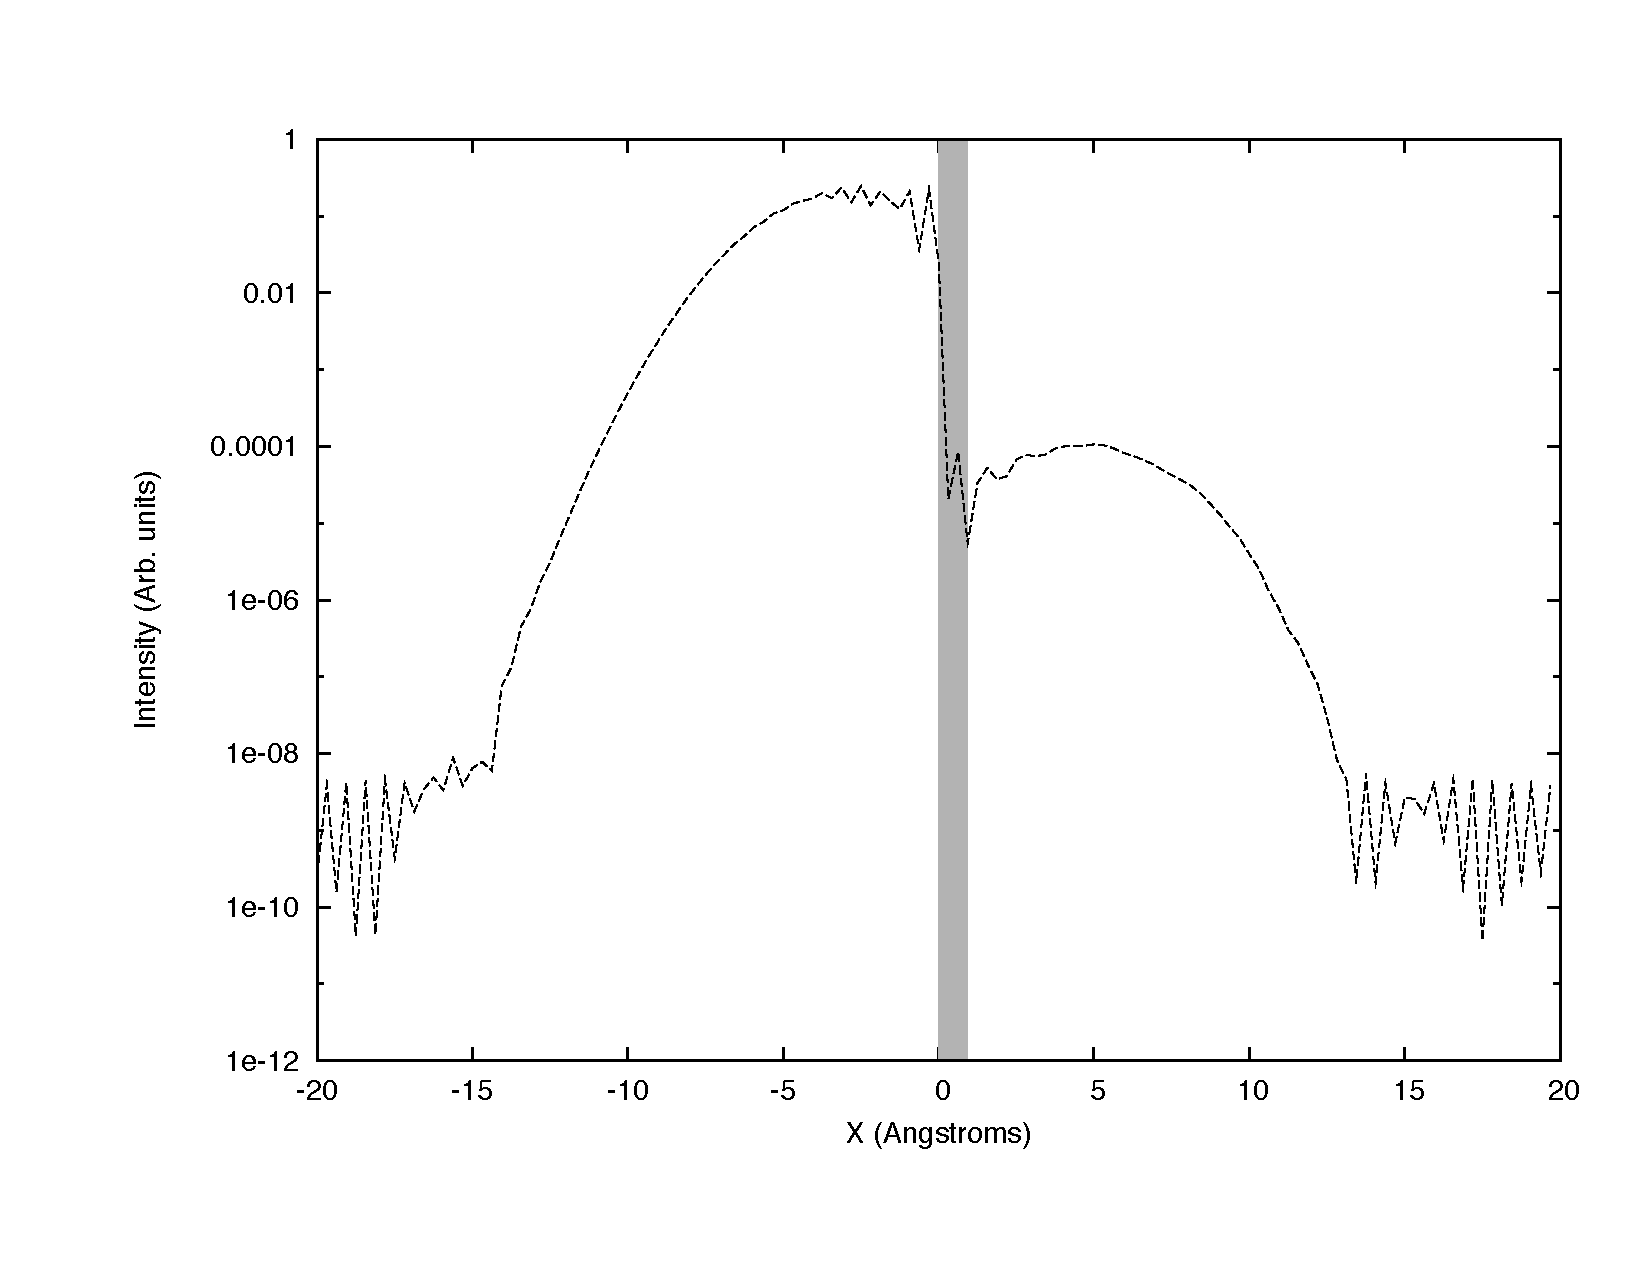
\includegraphics[width =120 mm, height = 95mm]{Ex_7_28_reflec.pdf}
\caption{Reflection and transmission of the wave packet after meeting the barrier.  Note the log scale to show the transmitted portion of the wave.}
\label{fig:728r}
\end{figure}
\begin{figure}[!h]
\centering
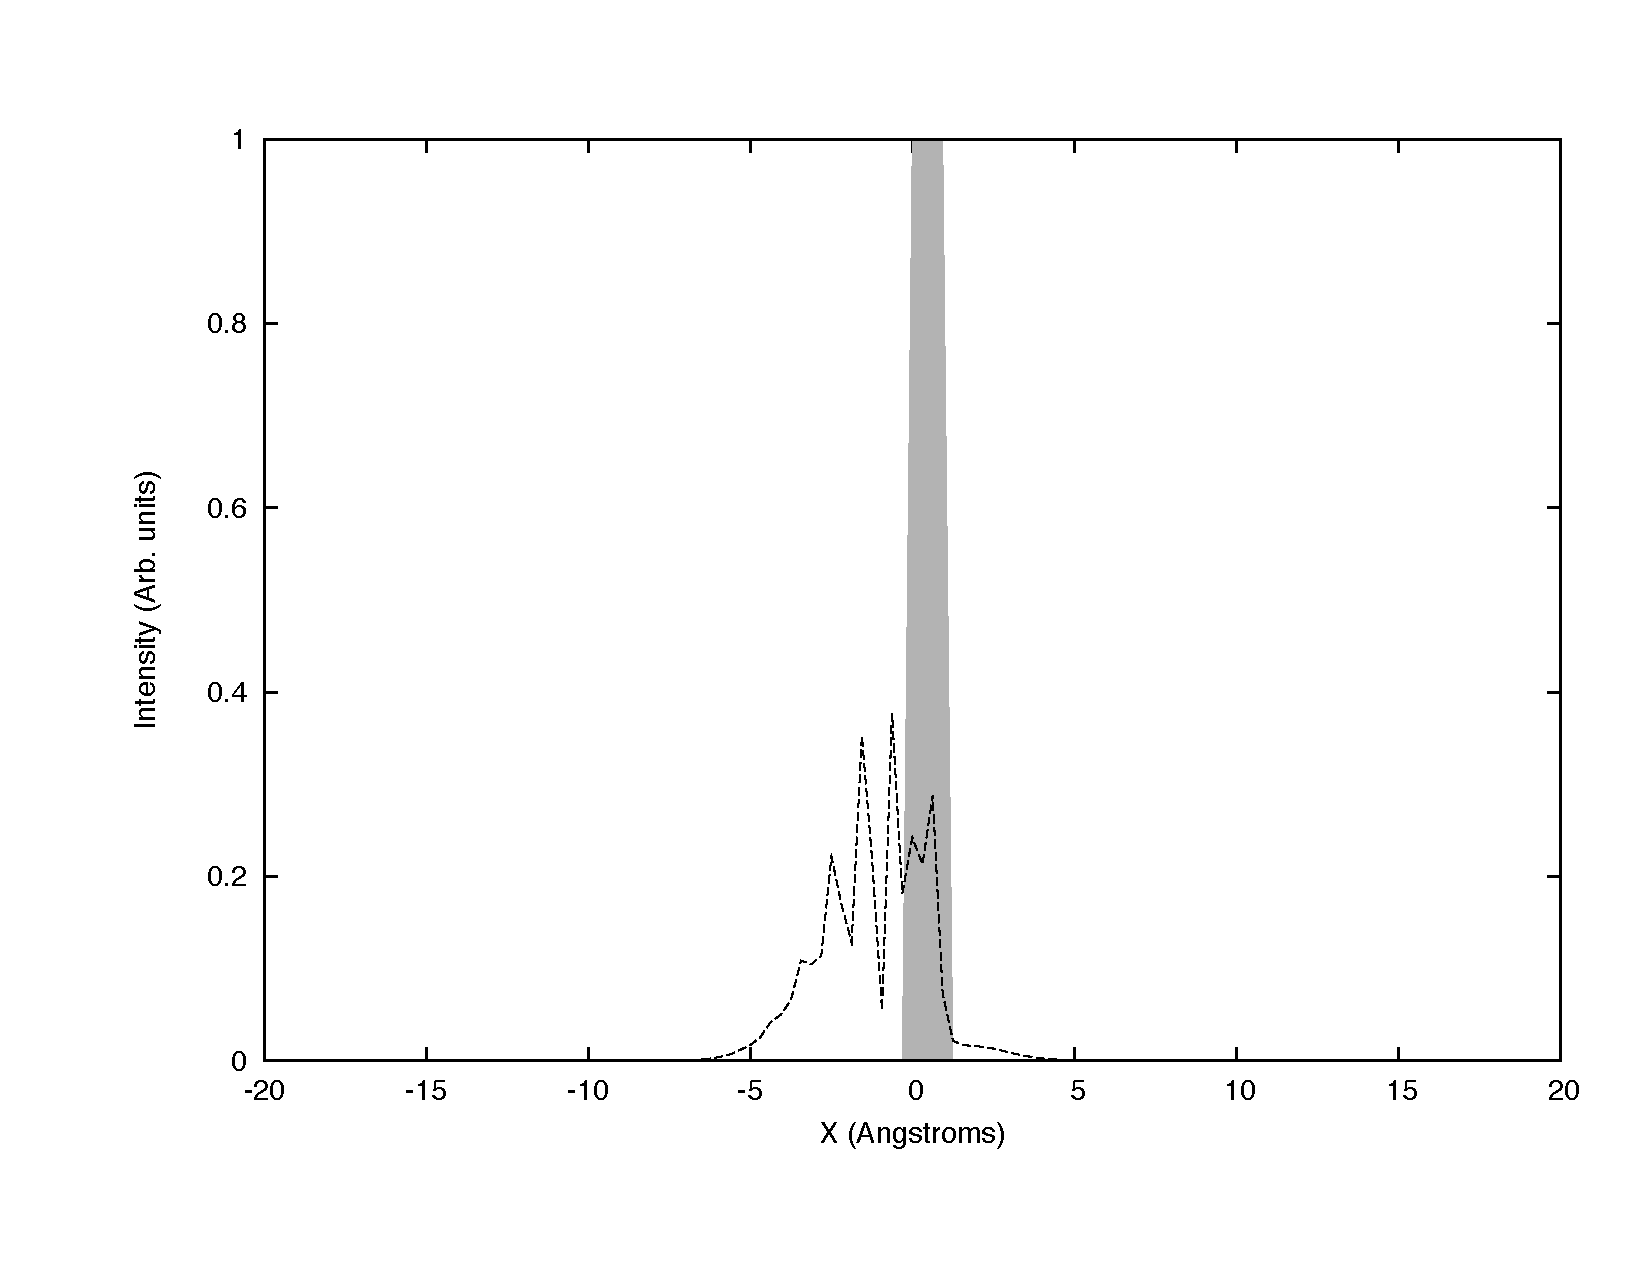
\includegraphics[width =120 mm, height = 95mm]{Ex_7_29_collis.pdf}
\caption{Wave packet meeting a thin potential barrier with energy greater than the barrier.}
\label{fig:729c}
\end{figure}
\begin{figure}[!h]
\centering
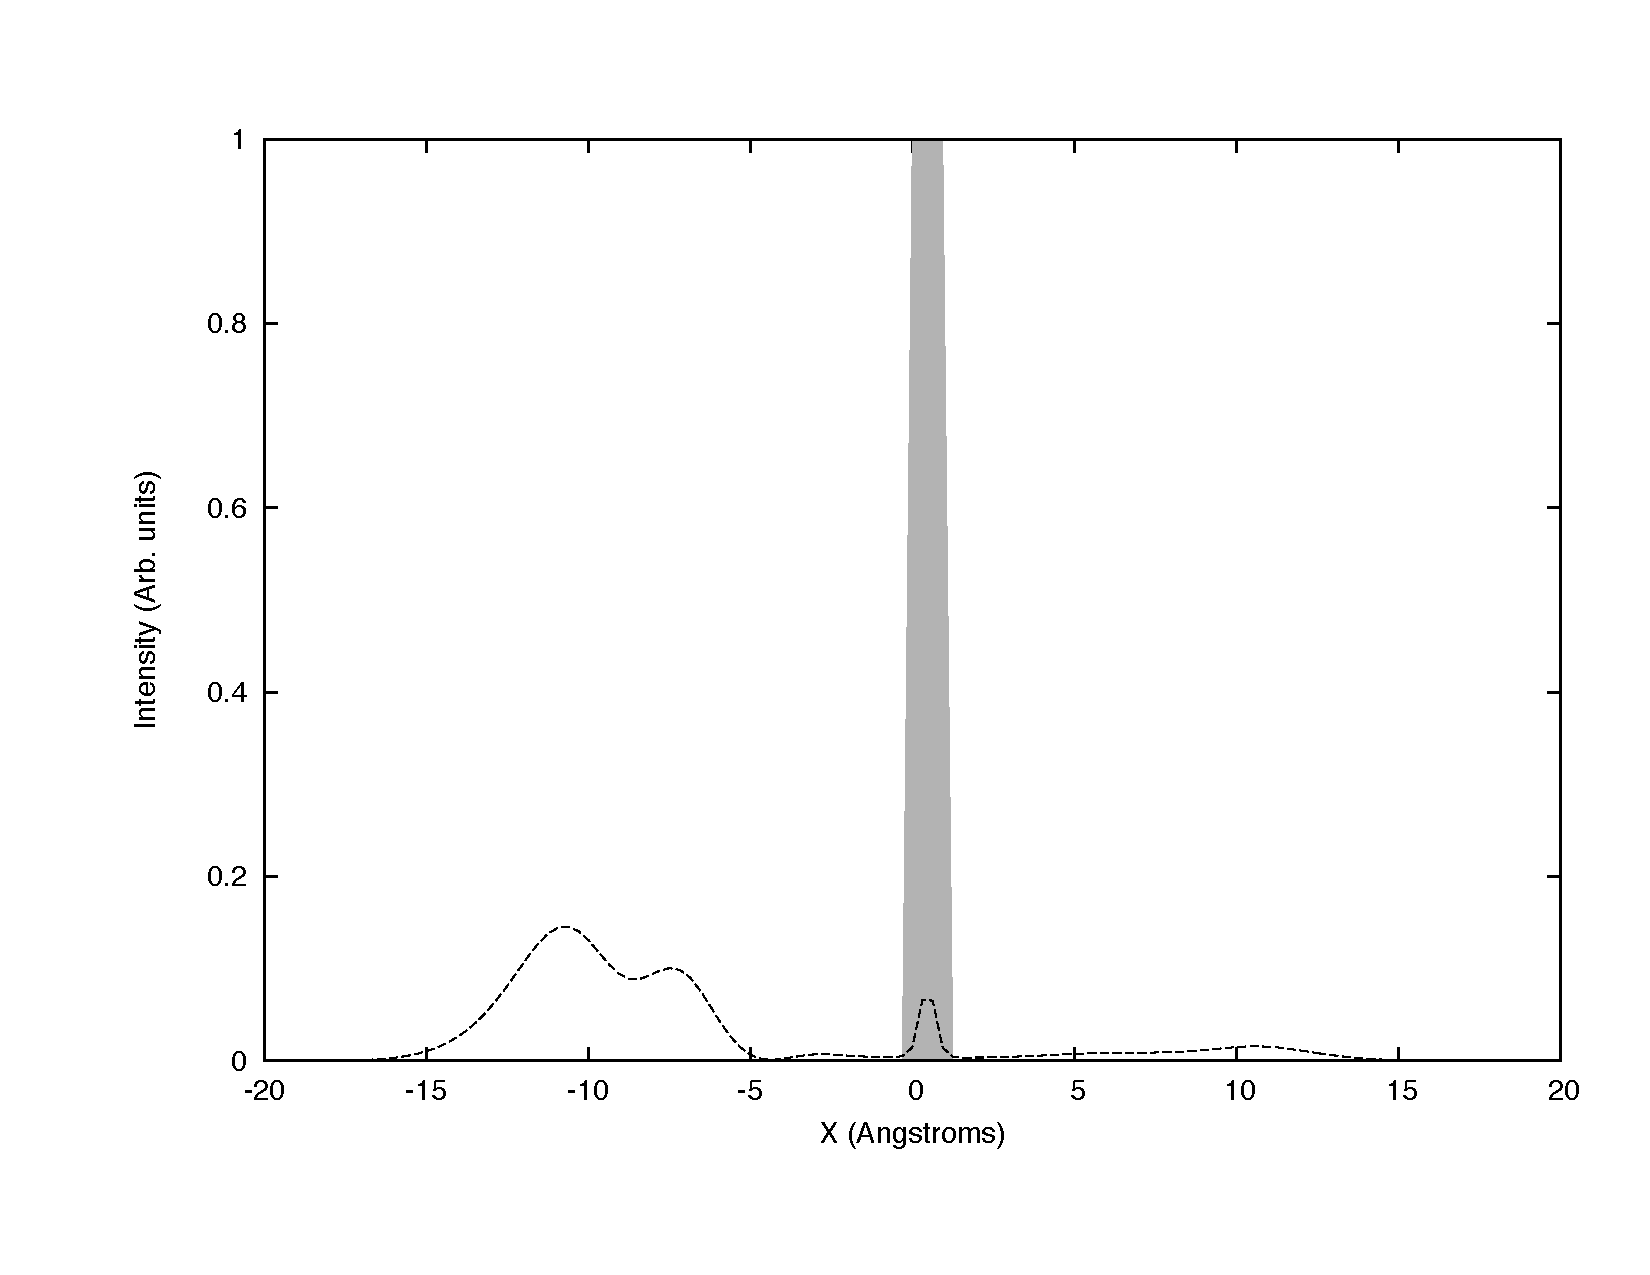
\includegraphics[width =120 mm, height = 95mm]{Ex_7_29_reflec.pdf}
\caption{Reflection and transmission of the wave packet after passing through the potential barrier.}
\label{fig:729r}
\end{figure}

\subsection{Radar/Sonar Ranging}
The final application to Fourier techniques was the analysis of simulated signal reflections for use in ranging via sonar or radar.  To begin this simulation, an initial signal was generated in the form of a pure sine wave for 20 seconds.  This signal is shown in Fig. \ref{fig:625init}.  This signal was then simulated to propagate through space and encounter a scatterer.  The reflected signal was then detected, but random noise was included to simulate a real world system.  This signal was then analyzed with cross correlation to select the signal from the noise.  Several different $c$ values were used to explore how this effected the quality of signal recognition, shown if Fig. \ref{fig:625} through \ref{fig:6255}.  As the value of $c$ is increased, the signal becomes more pronounced at its center, but one loses information about the width of the reflected signal.  This is not a particularly significant drawback, since one knows the size of the outgoing signal when it is generated.
\begin{figure}[!h]
\centering
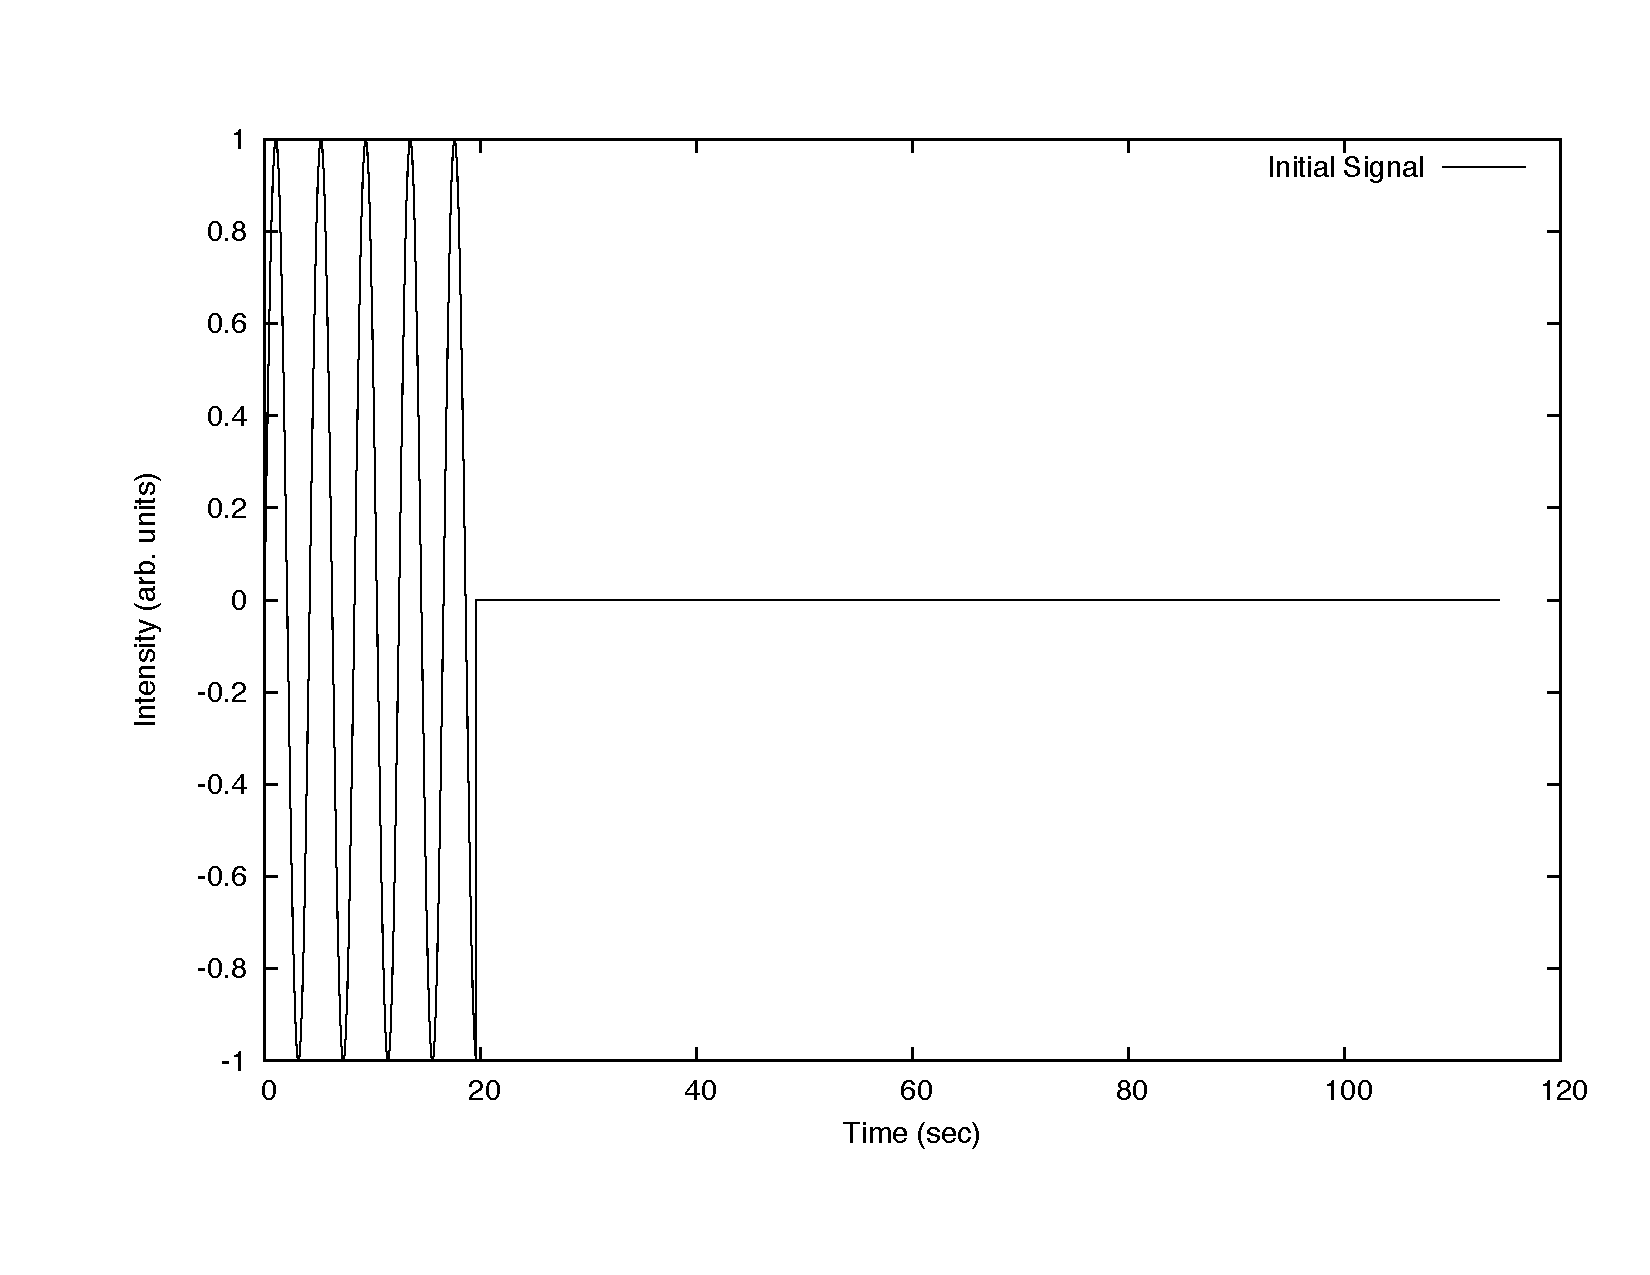
\includegraphics[width =120 mm, height = 95mm]{Ex_6_25_init.pdf}
\caption{Generated signal transmitted towards the reflector.}
\label{fig:625init}
\end{figure}
\begin{figure}[!h]
\centering
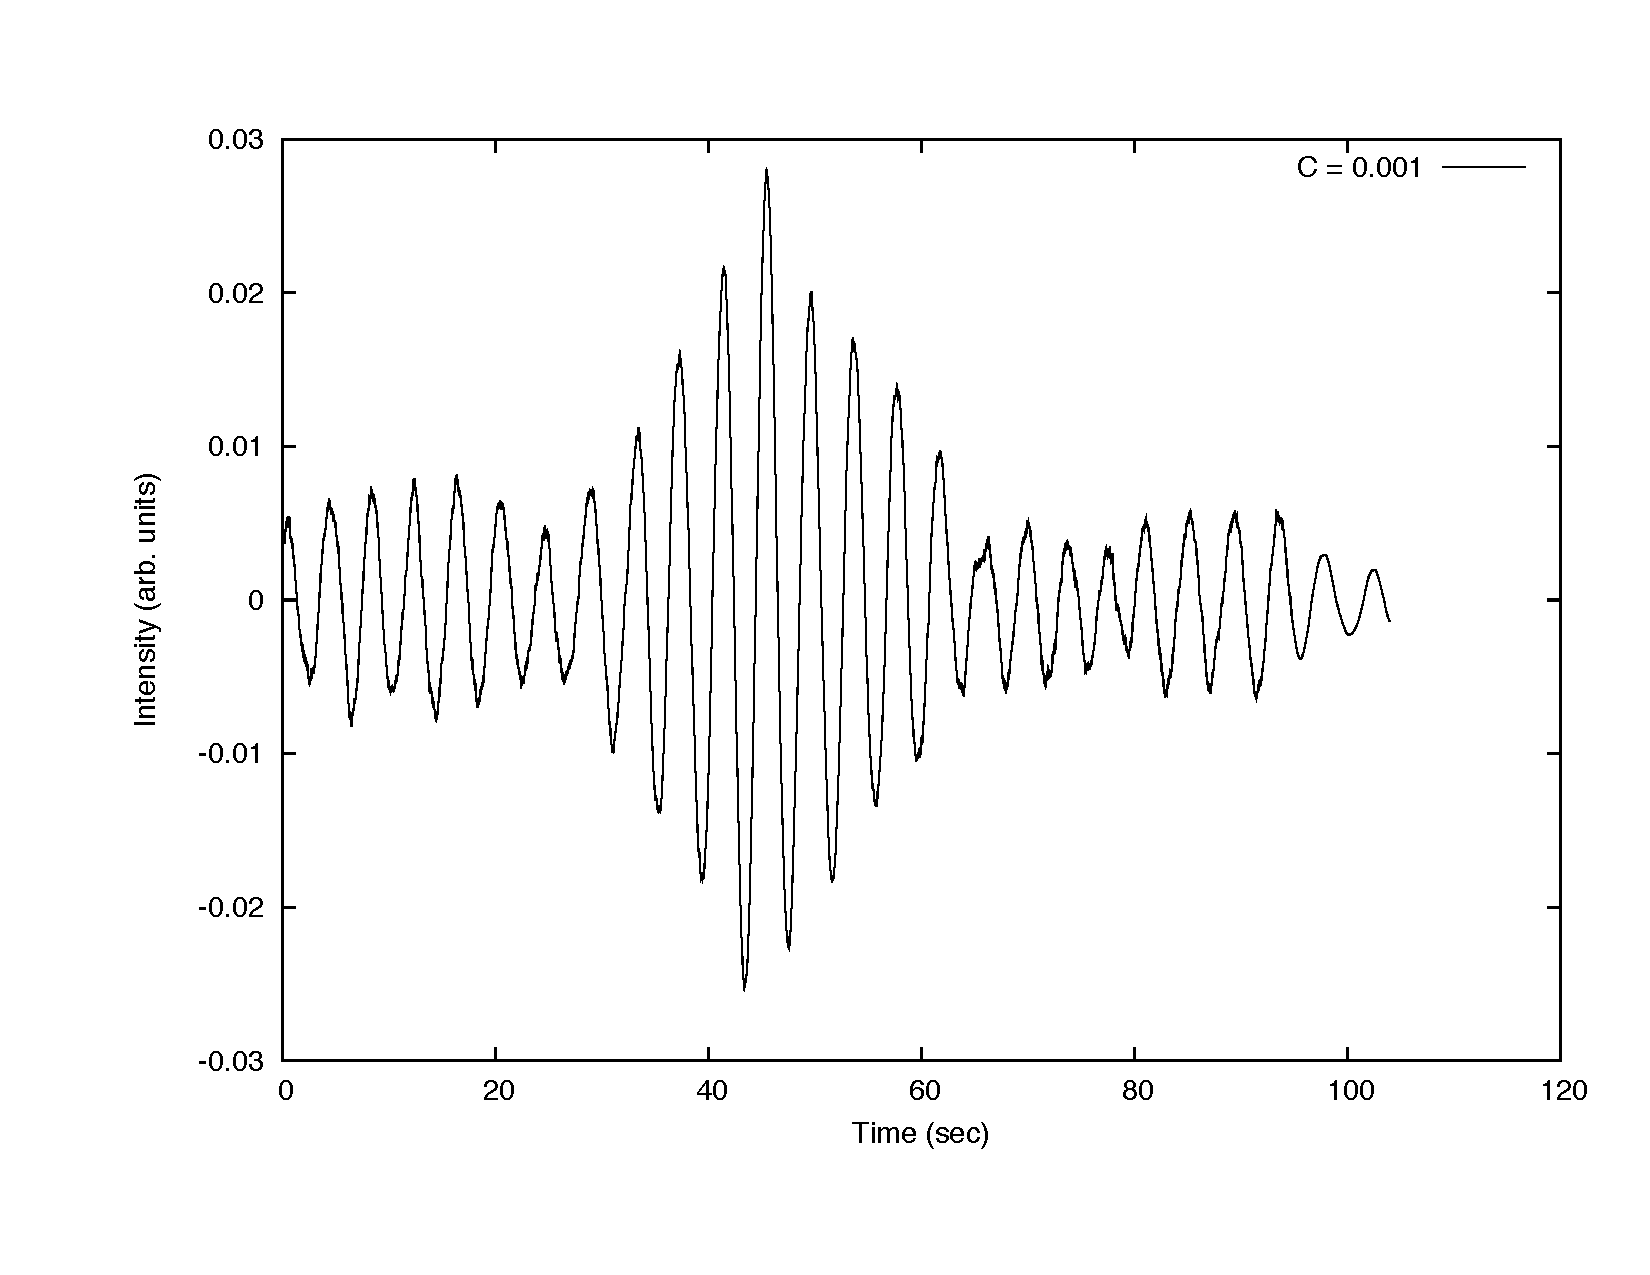
\includegraphics[width =120 mm, height = 95mm]{Ex_6_25_cross.pdf}
\caption{Cross correlation with $c=0.001$.}
\label{fig:625}
\end{figure}
\begin{figure}[!h]
\centering
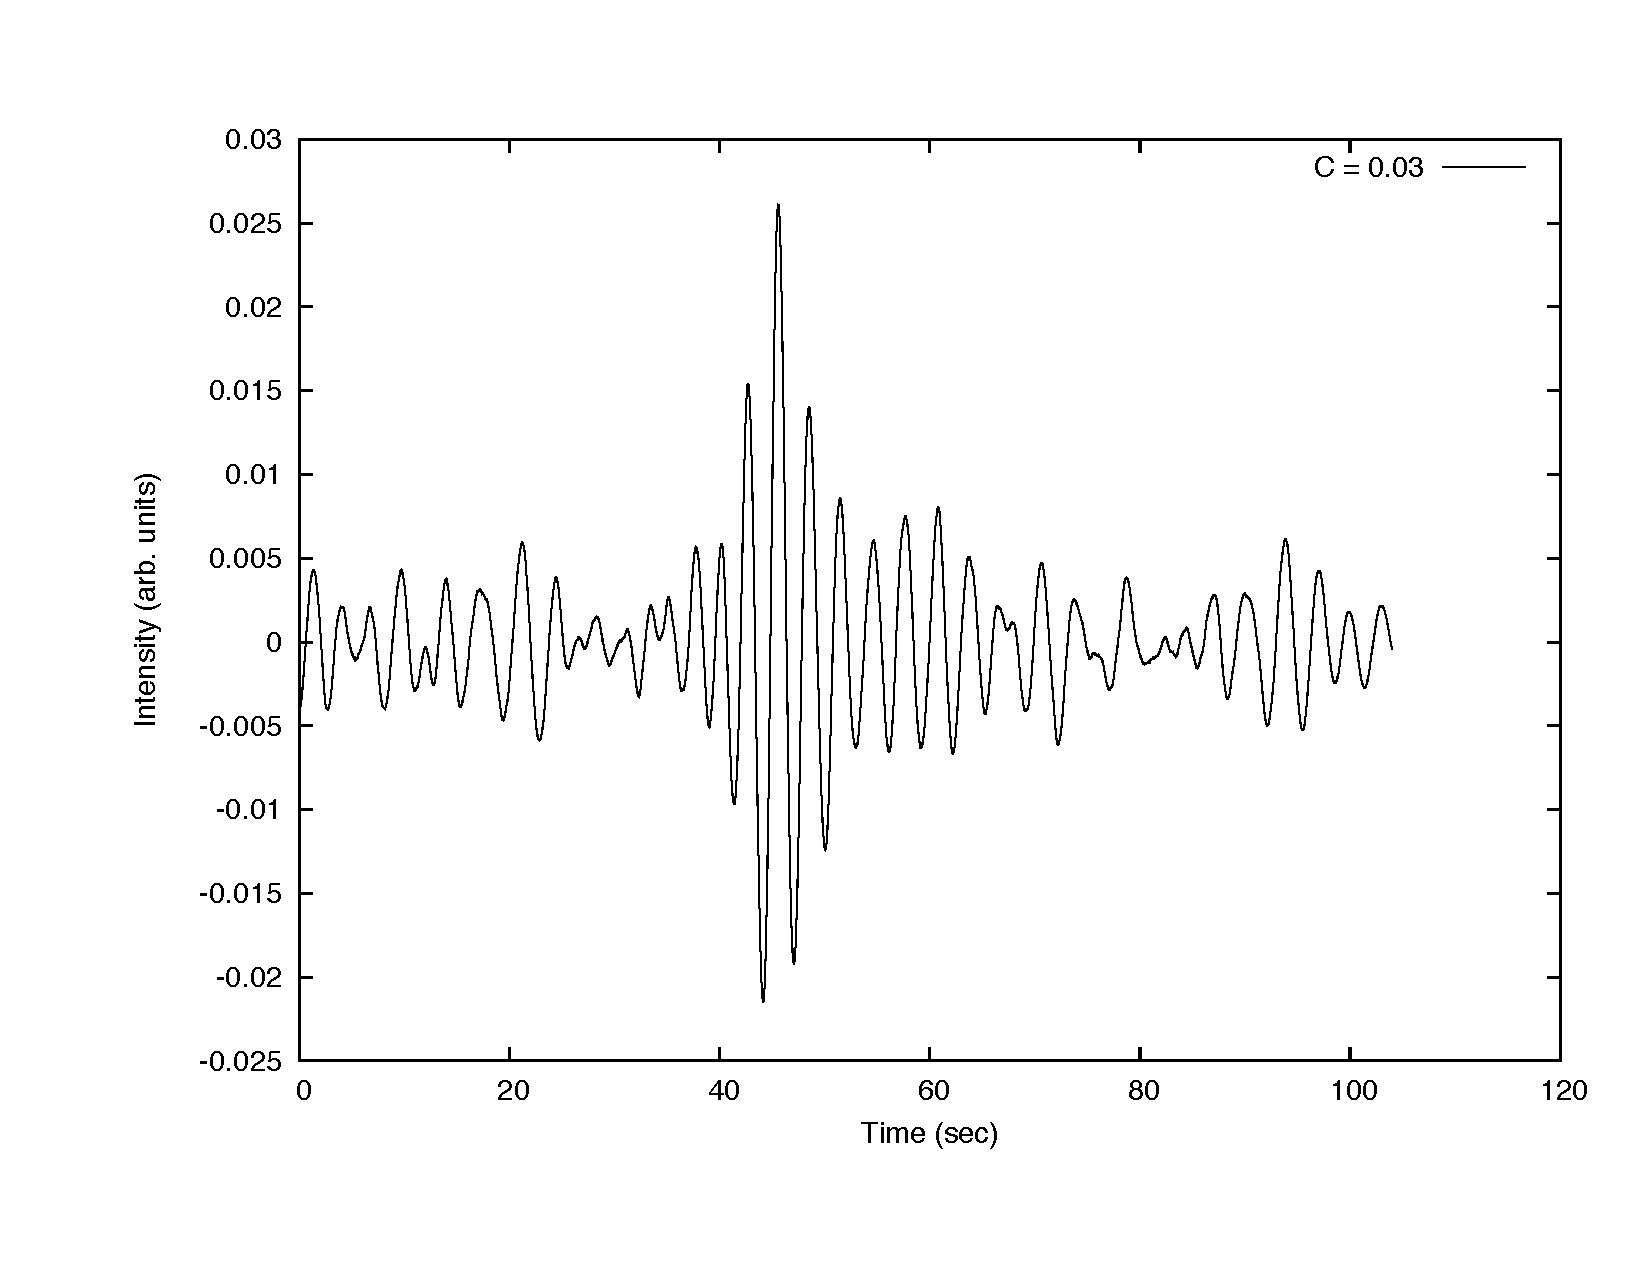
\includegraphics[width =120 mm, height = 95mm]{Ex_6_25_cross3.pdf}
\caption{Cross correlation with $c=0.03$.}
\label{fig:6253}
\end{figure}
\begin{figure}[!h]
\centering
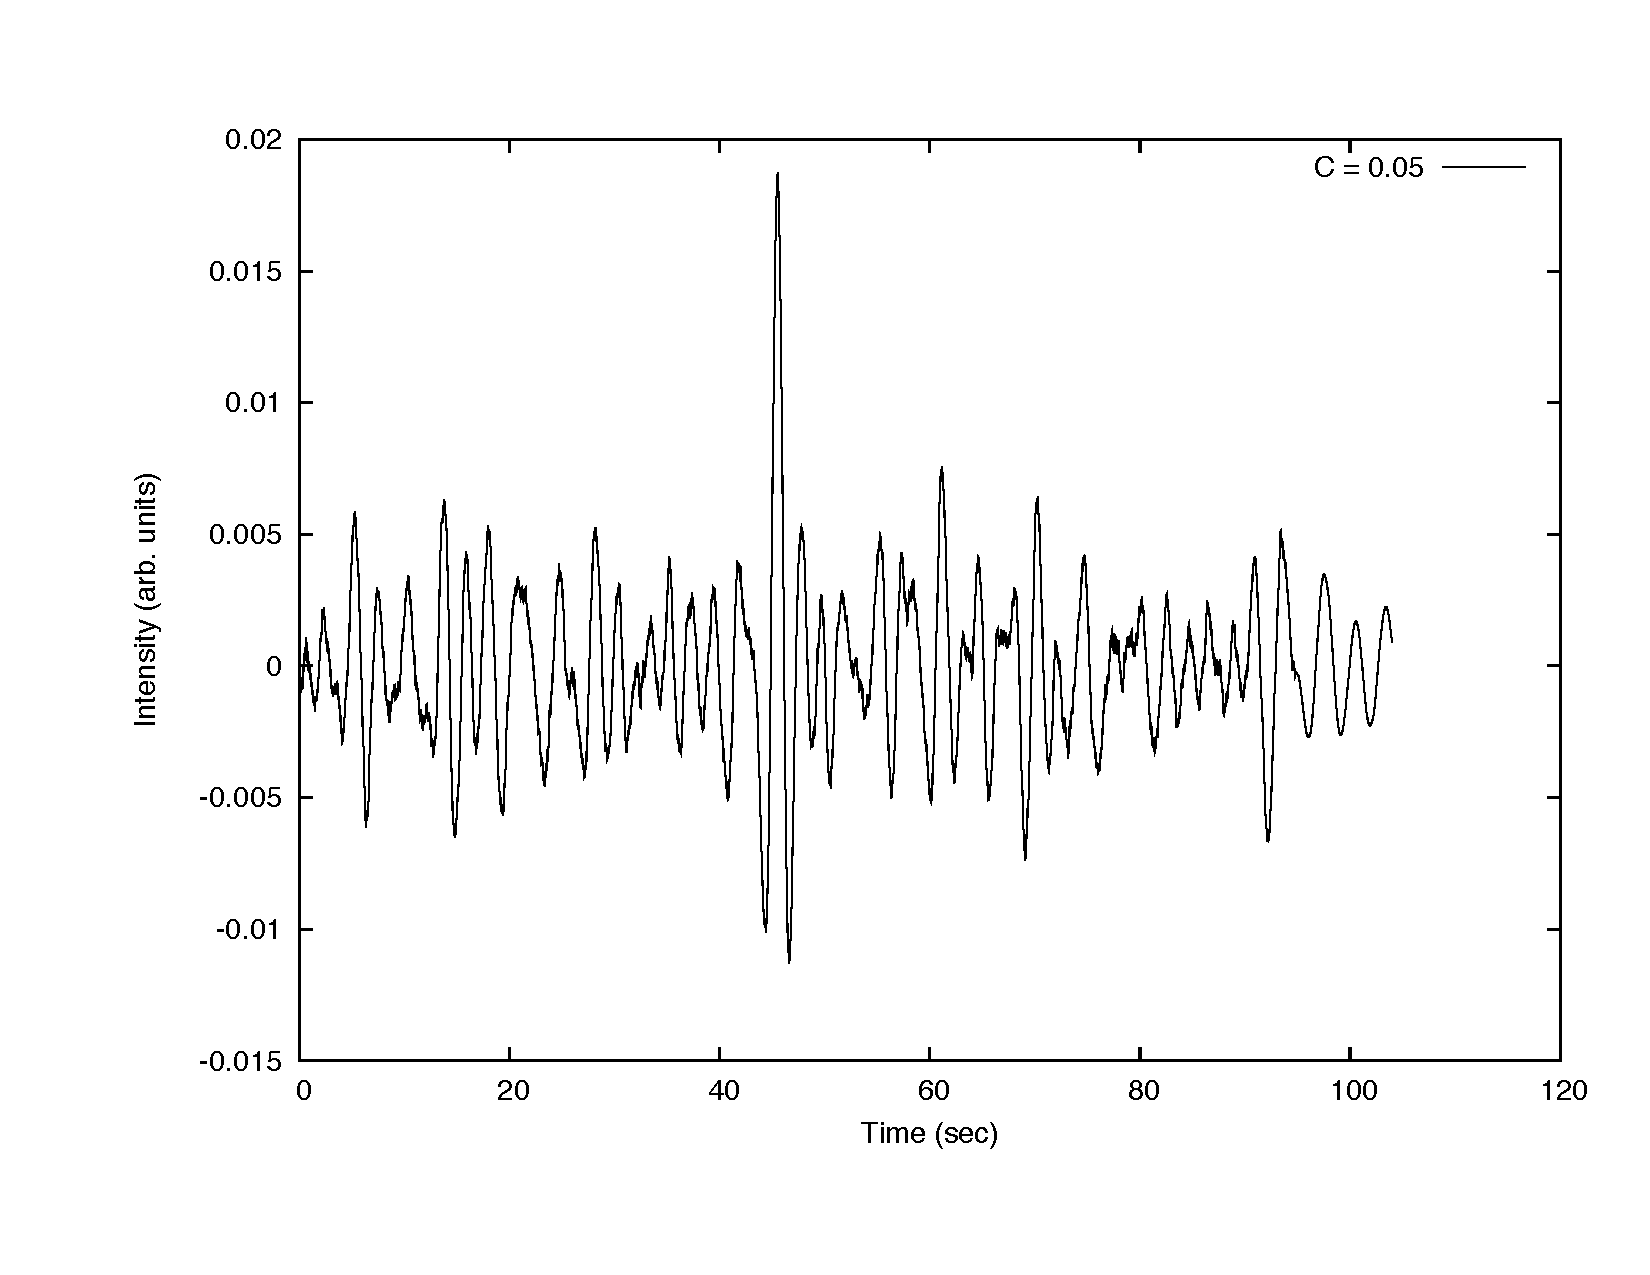
\includegraphics[width =120 mm, height = 95mm]{Ex_6_25_cross5.pdf}
\caption{Cross correlation with $c=0.05$.}
\label{fig:6255}
\end{figure}

Next, a signal was simulated to contain two different reflectors.  Again, several different $c$ values were used.  This simulation clearly demonstrates the properties discussed above.  At low $c$, there is no clear signal coming through the noise.  However, at $c=0.05$, one observes two very distinct peaks, corresponding to the two different reflectors.

\begin{figure}[!h]
\centering
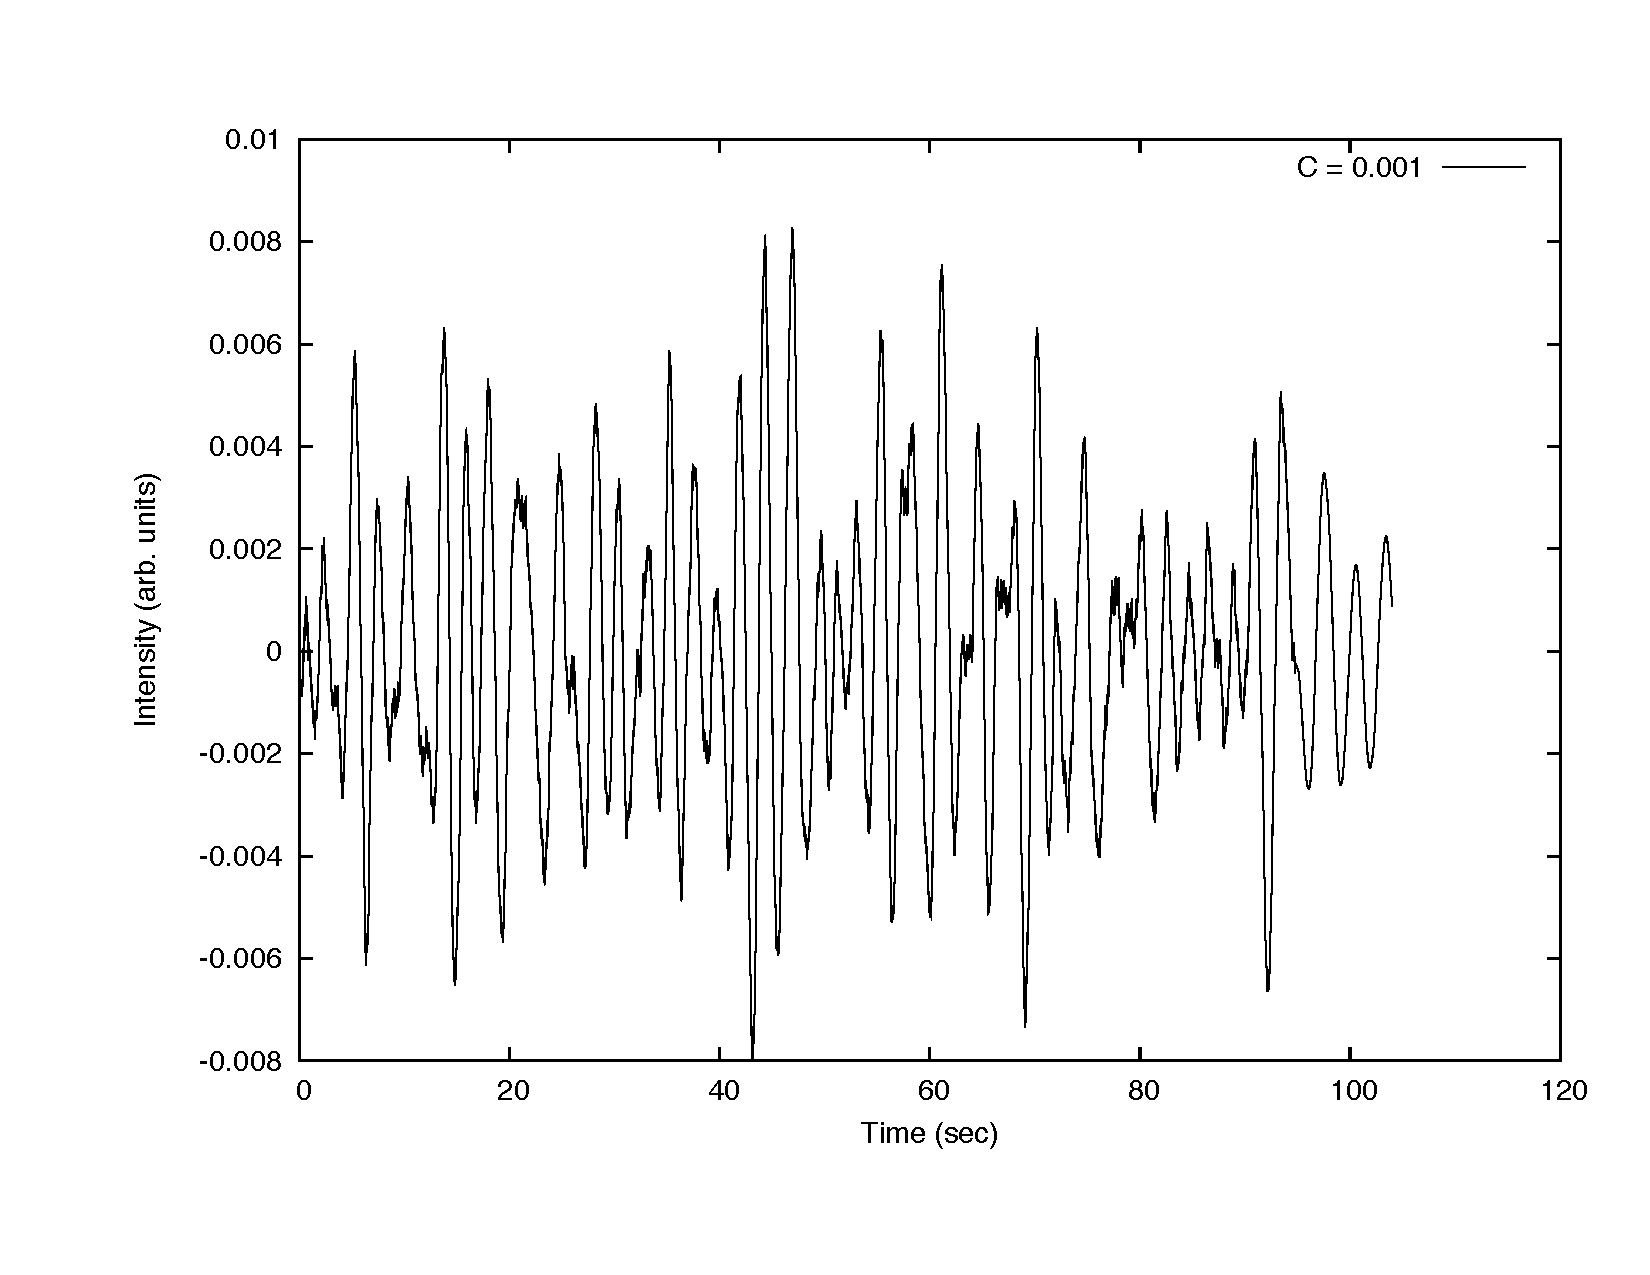
\includegraphics[width =120 mm, height = 95mm]{Ex_6_26_cross.pdf}
\caption{Cross correlation with $c=0.001$.}
\label{fig:626}
\end{figure}
\begin{figure}[!h]
\centering
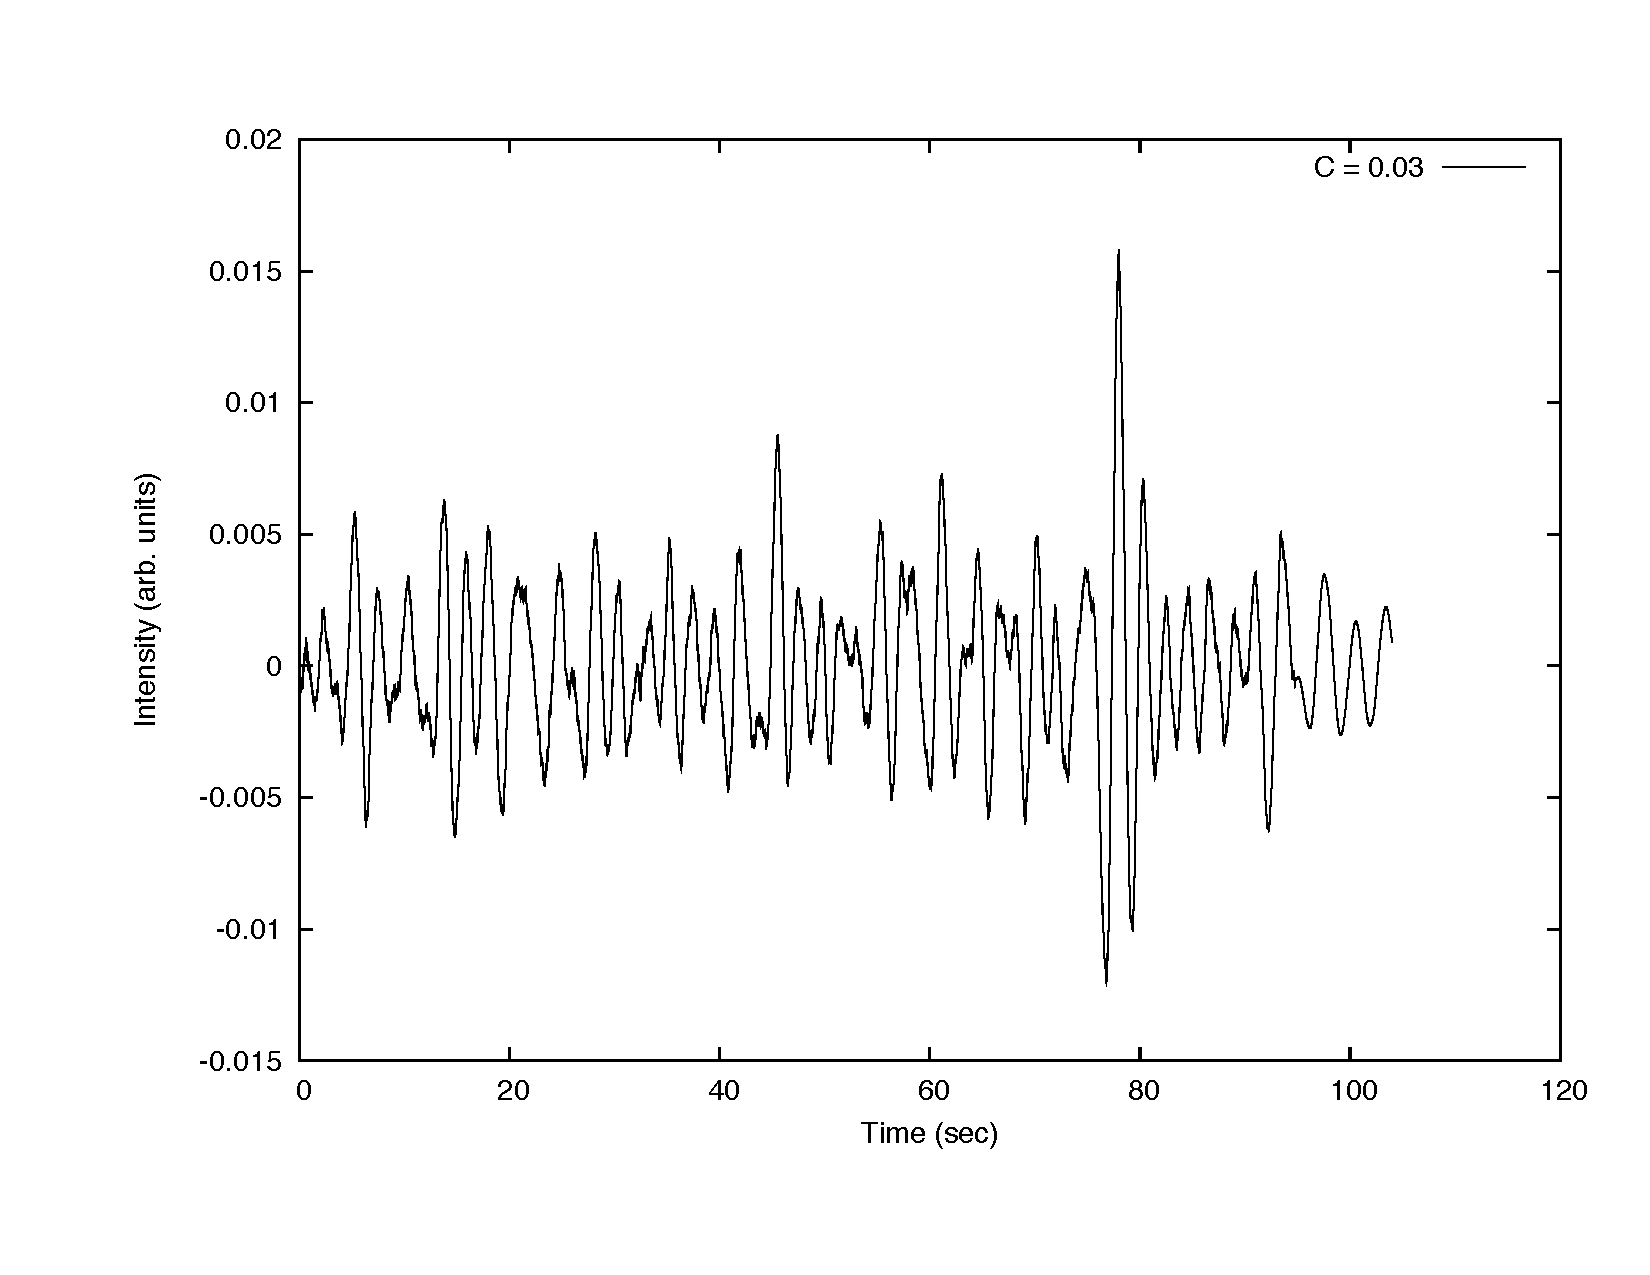
\includegraphics[width =120 mm, height = 95mm]{Ex_6_26_cross3.pdf}
\caption{Cross correlation with $c=0.03$.}
\label{fig:6263}
\end{figure}
\begin{figure}[!h]
\centering
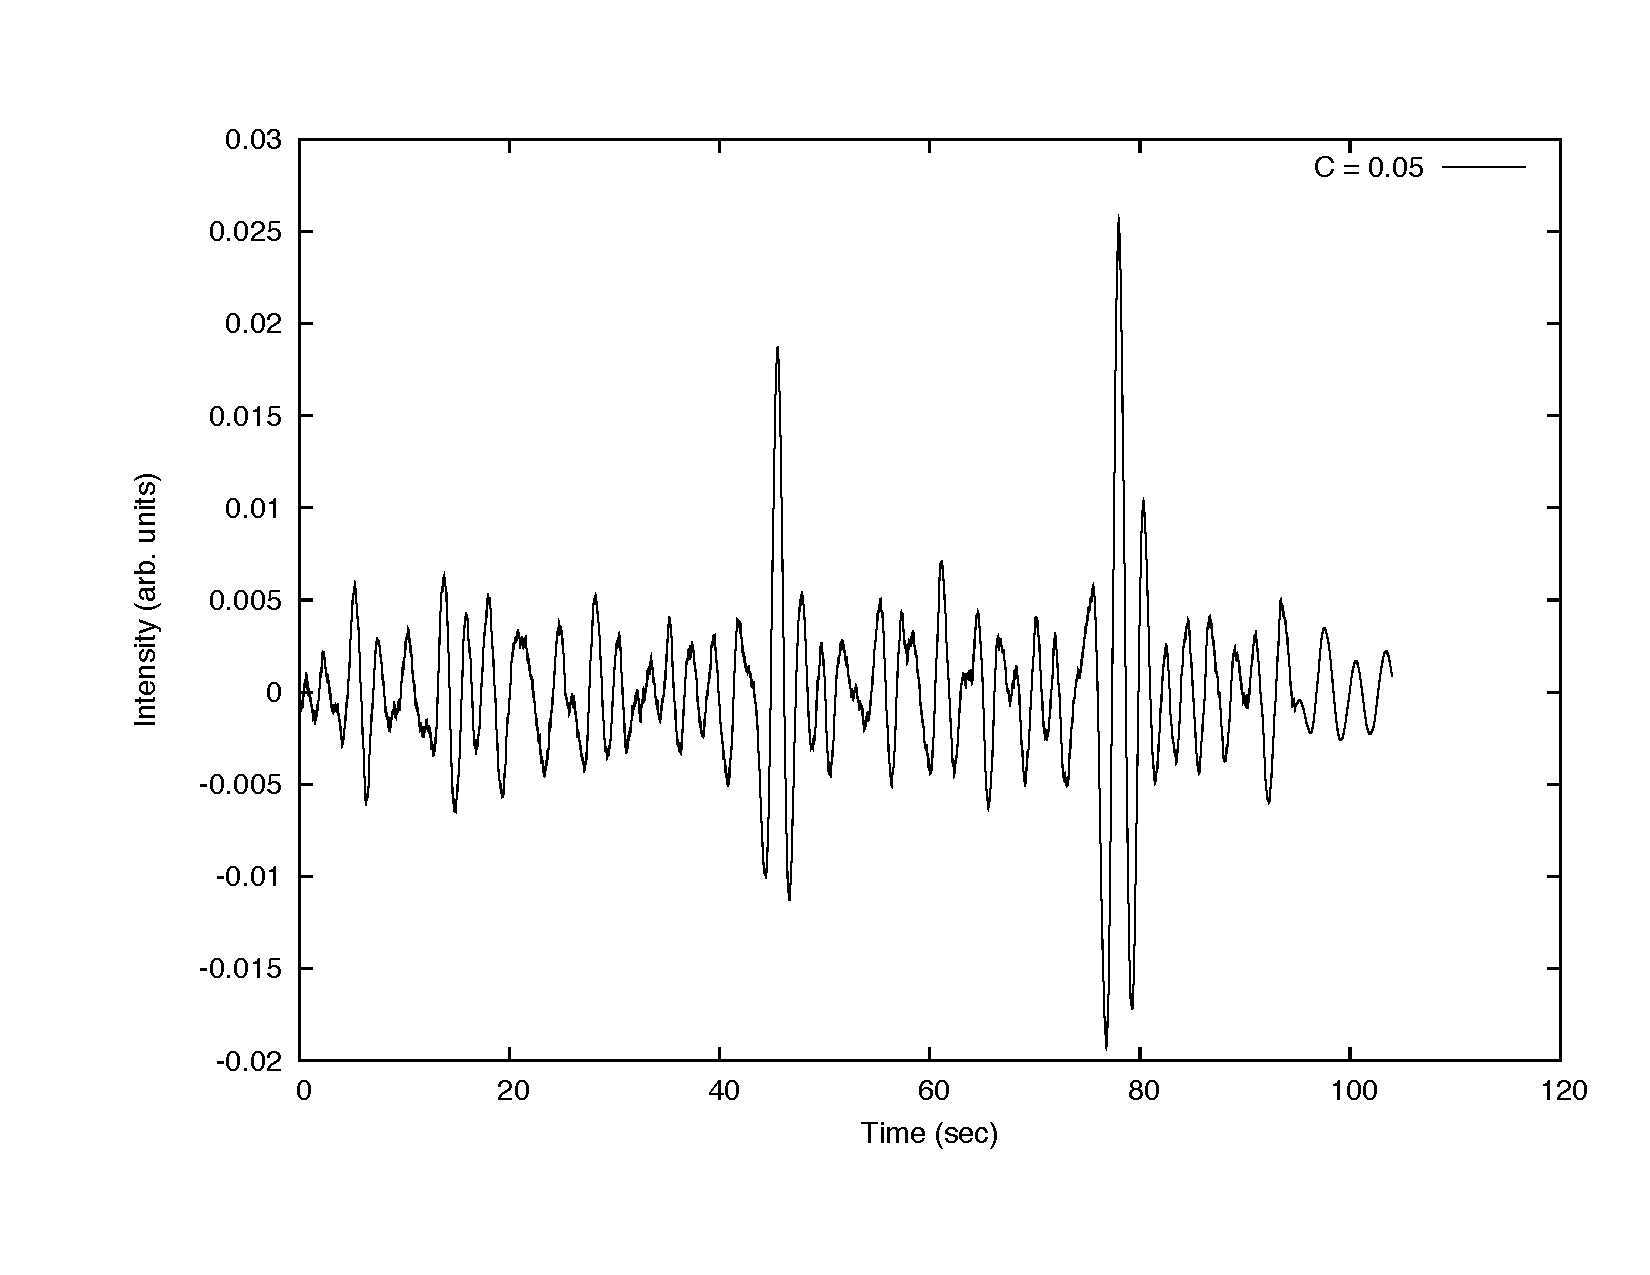
\includegraphics[width =120 mm, height = 95mm]{Ex_6_26_cross5.pdf}
\caption{Cross correlation with $c=0.05$.}
\label{fig:6265}
\end{figure}



\end{document}

